% Options for packages loaded elsewhere
\PassOptionsToPackage{unicode}{hyperref}
\PassOptionsToPackage{hyphens}{url}
%
\documentclass[
  11pt,
  a4paper]{article}
\usepackage{amsmath,amssymb}
\usepackage{lmodern}
\usepackage{ifxetex,ifluatex}
\ifnum 0\ifxetex 1\fi\ifluatex 1\fi=0 % if pdftex
  \usepackage[T1]{fontenc}
  \usepackage[utf8]{inputenc}
  \usepackage{textcomp} % provide euro and other symbols
\else % if luatex or xetex
  \usepackage{unicode-math}
  \defaultfontfeatures{Scale=MatchLowercase}
  \defaultfontfeatures[\rmfamily]{Ligatures=TeX,Scale=1}
\fi
% Use upquote if available, for straight quotes in verbatim environments
\IfFileExists{upquote.sty}{\usepackage{upquote}}{}
\IfFileExists{microtype.sty}{% use microtype if available
  \usepackage[]{microtype}
  \UseMicrotypeSet[protrusion]{basicmath} % disable protrusion for tt fonts
}{}
\makeatletter
\@ifundefined{KOMAClassName}{% if non-KOMA class
  \IfFileExists{parskip.sty}{%
    \usepackage{parskip}
  }{% else
    \setlength{\parindent}{0pt}
    \setlength{\parskip}{6pt plus 2pt minus 1pt}}
}{% if KOMA class
  \KOMAoptions{parskip=half}}
\makeatother
\usepackage{xcolor}
\IfFileExists{xurl.sty}{\usepackage{xurl}}{} % add URL line breaks if available
\IfFileExists{bookmark.sty}{\usepackage{bookmark}}{\usepackage{hyperref}}
\hypersetup{
  pdftitle={High resolution, annual maps of field boundaries for smallholder-dominated croplands at national scales},
  pdfkeywords={rmarkdown, reproducible science},
  hidelinks,
  pdfcreator={LaTeX via pandoc}}
\urlstyle{same} % disable monospaced font for URLs
\usepackage[margin=1in]{geometry}
\usepackage{longtable,booktabs,array}
\usepackage{calc} % for calculating minipage widths
% Correct order of tables after \paragraph or \subparagraph
\usepackage{etoolbox}
\makeatletter
\patchcmd\longtable{\par}{\if@noskipsec\mbox{}\fi\par}{}{}
\makeatother
% Allow footnotes in longtable head/foot
\IfFileExists{footnotehyper.sty}{\usepackage{footnotehyper}}{\usepackage{footnote}}
\makesavenoteenv{longtable}
\usepackage{graphicx}
\makeatletter
\def\maxwidth{\ifdim\Gin@nat@width>\linewidth\linewidth\else\Gin@nat@width\fi}
\def\maxheight{\ifdim\Gin@nat@height>\textheight\textheight\else\Gin@nat@height\fi}
\makeatother
% Scale images if necessary, so that they will not overflow the page
% margins by default, and it is still possible to overwrite the defaults
% using explicit options in \includegraphics[width, height, ...]{}
\setkeys{Gin}{width=\maxwidth,height=\maxheight,keepaspectratio}
% Set default figure placement to htbp
\makeatletter
\def\fps@figure{htbp}
\makeatother
\setlength{\emergencystretch}{3em} % prevent overfull lines
\providecommand{\tightlist}{%
  \setlength{\itemsep}{0pt}\setlength{\parskip}{0pt}}
\setcounter{secnumdepth}{5}
% Allowing for landscape pages
\usepackage{lscape}
\usepackage{graphicx}
\newcommand{\blandscape}{\begin{landscape}}
\newcommand{\elandscape}{\end{landscape}}

% Left justification of the text: see https://www.sharelatex.com/learn/Text_alignment
% \usepackage[document]{ragged2e} % already in the latex template
\newcommand{\bleft}{\begin{flushleft}}
\newcommand{\eleft}{\end{flushleft}}
\usepackage{float}
\usepackage{titling}
\usepackage{setspace}
\usepackage{booktabs}
\usepackage{longtable}
\usepackage{array}
\usepackage{multirow}
\usepackage{wrapfig}
\usepackage{colortbl}
\usepackage{pdflscape}
\usepackage{tabu}
\usepackage{threeparttable}
\usepackage{threeparttablex}
\usepackage[normalem]{ulem}
\usepackage{makecell}
\usepackage{xcolor}
\ifluatex
  \usepackage{selnolig}  % disable illegal ligatures
\fi
\newlength{\cslhangindent}
\setlength{\cslhangindent}{1.5em}
\newlength{\csllabelwidth}
\setlength{\csllabelwidth}{3em}
\newenvironment{CSLReferences}[2] % #1 hanging-ident, #2 entry spacing
 {% don't indent paragraphs
  \setlength{\parindent}{0pt}
  % turn on hanging indent if param 1 is 1
  \ifodd #1 \everypar{\setlength{\hangindent}{\cslhangindent}}\ignorespaces\fi
  % set entry spacing
  \ifnum #2 > 0
  \setlength{\parskip}{#2\baselineskip}
  \fi
 }%
 {}
\usepackage{calc}
\newcommand{\CSLBlock}[1]{#1\hfill\break}
\newcommand{\CSLLeftMargin}[1]{\parbox[t]{\csllabelwidth}{#1}}
\newcommand{\CSLRightInline}[1]{\parbox[t]{\linewidth - \csllabelwidth}{#1}\break}
\newcommand{\CSLIndent}[1]{\hspace{\cslhangindent}#1}

\title{High resolution, annual maps of field boundaries for
smallholder-dominated croplands at national scales}
\usepackage{etoolbox}
\makeatletter
\providecommand{\subtitle}[1]{% add subtitle to \maketitle
  \apptocmd{\@title}{\par {\large #1 \par}}{}{}
}
\makeatother
\subtitle{Supporting Information}
\author{}
\date{\vspace{-2.5em}}

\begin{document}
\maketitle

{
\setcounter{tocdepth}{4}
\tableofcontents
}
\newcommand{\beginsupplement}{%
        \setcounter{table}{0}
        \renewcommand{\thetable}{S\arabic{table}}%
        \setcounter{figure}{0}
        \renewcommand{\thefigure}{S\arabic{figure}}%
     }

%
        \setcounter{table}{0}
        \renewcommand{\thetable}{S\arabic{table}}%
        \setcounter{figure}{0}
        \renewcommand{\thefigure}{S\arabic{figure}}%
     
\singlespace

\bleft

\hypertarget{code-and-data-availability}{%
\section{Code and Data Availability}\label{code-and-data-availability}}

The repositories containing the data, code, and manuscript source files
used to produce this paper are listed below:

\begin{itemize}
\tightlist
\item
  \href{https://github.com/agroimpacts/activemapper}{\texttt{activemapper}}:
  Repository\footnote{github.com/agroimpacts/activemapper} containing
  code and derived data used to write this paper.
\item
  \href{https:github.com/agroimpacts/imager}{\texttt{imager}}:
  Repository\footnote{github.com/agroimpacts/imager} containing code for
  the image processing software.
\item
  \href{https:github.com/agroimpacts/labeller}{\texttt{labeller}}:
  Repository\footnote{github.com/agroimpacts/labeller} containing code
  for the labelling platform.
\item
  \href{https:github.com/agroimpacts/learner}{\texttt{learner}}:
  Repository\footnote{github.com/agroimpacts/learner} containing code
  for the active learning component.
\item
  \href{https:github.com/agroimpacts/segmenter}{\texttt{segmenter}}:
  Repository\footnote{github.com/agroimpacts/segmenter} containing code
  for the segmentation algorithm.
\item
  \href{https://mappingafrica.io}{\texttt{mappingafrica.io}}: Project
  website\footnote{https://mappingafrica.io} linking to web map
  displaying field boundary maps. The web map is currently undergoing
  redevelopment, and will be hosted on a new URL and links download
  maps. In the interim, map data are available on request.
\end{itemize}

\hypertarget{supplemental-methods}{%
\section{Supplemental Methods}\label{supplemental-methods}}

\hypertarget{map-reference-system}{%
\subsection{Map reference system}\label{map-reference-system}}

The map reference system used in our mapping approach had three
different levels. At the coarsest level, Ghana was divided into 16
different mapping zones, or areas of interest (AOIS; Figure
\ref{fig:aois}A), that were used to create AOI-specific mapping models.
Each AOIs was comprised of 400 to 777 adjacent tiles. These tiles were
used to create seasonal image composites, and were defined within a 0.05
degree grid (Figure \ref{fig:aois}B)), with each tile numbered to
correspond to a larger 1 degree grid cell that it sits within (dotted
lines in Figure \ref{fig:aois}B). Training and reference labels were
created within a 0.005 degree grid that nested within each tile (Figure
\ref{fig:aois}C). Therefore, each tile has 100 grid cells, and there are
400 tiles per 1X1 degree. The smallest AOI consists of a single 1X1
degree, which fall in the center of the country (AOIs 5, 8, 11, and 14).
AOIs falling along Ghana's boundaries were created by tiles from 1X1
degree cells that straddled Ghana's border with those from the closest
degree cells that were fully contained within Ghana (e.g.~AOI 1), with
the exception of AOI 16, which was comprised of tiles in three partial
1X1 degree cells along Ghana's coast.

\begin{figure}[!ht]

{\centering 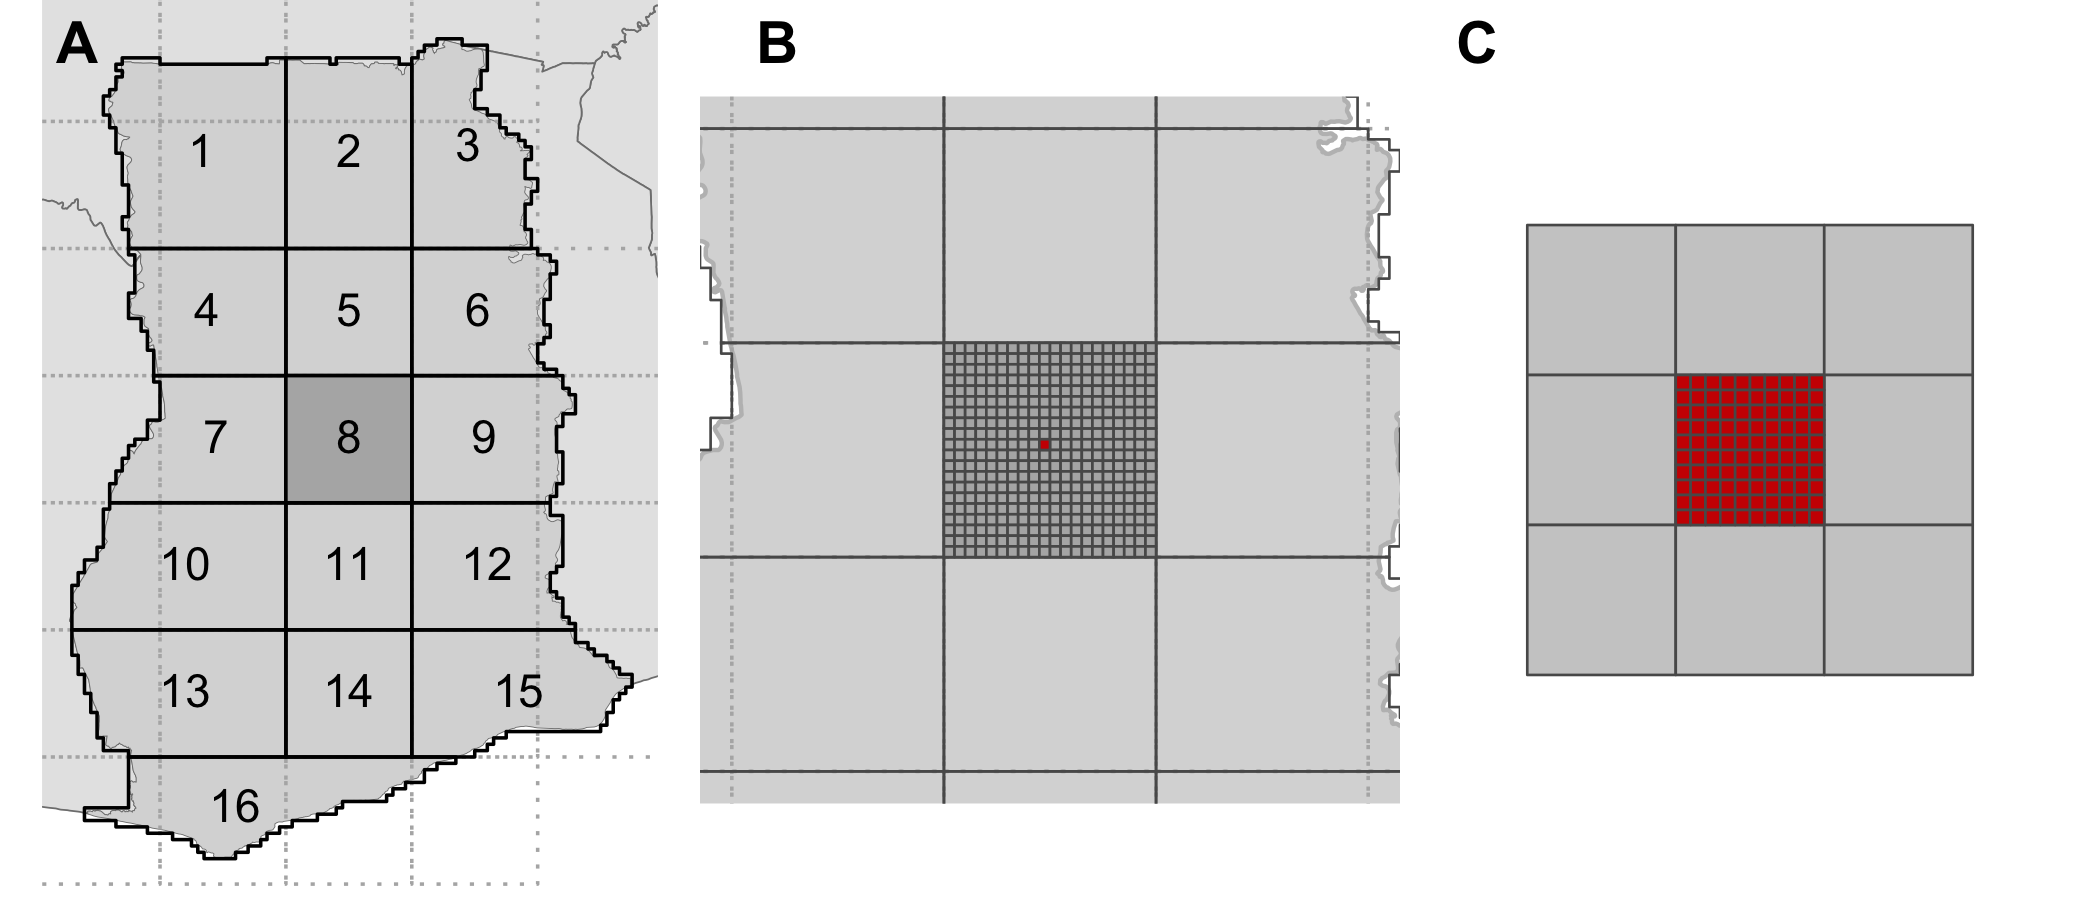
\includegraphics[width=1\linewidth,]{figures/reference_system} 

}

\caption{The reference system used in this mapping approach, including A) numbered areas of interest (AOIs) that define the minimum mapping geography (solid black lines; dotted lines indicate boundaries of 1 degree grid), B) the 0.05 degree tile used for compositing imagery, and C) the 0.005 degree resolution reference grid used for collecting training data and distributed computing.}\label{fig:aois}
\end{figure}

\hypertarget{image-compositing}{%
\subsection{Image compositing}\label{image-compositing}}

\hypertarget{variation-in-lengths-of-temporal-window-used}{%
\subsubsection{Variation in lengths of temporal window
used}\label{variation-in-lengths-of-temporal-window-used}}

The typical window for compositing dry season imagery was December, 2018
to February, 2019, but in the cloudiest regions (AOIs 10, 11, 13, 14,
16) we started the dry season window in November, to ensure a sufficient
density of images for compositing.

\hypertarget{assessing-composite-quality}{%
\subsubsection{Assessing composite
quality}\label{assessing-composite-quality}}

The rubric presented in Table \ref{tab:imqcriteria} was used to assess
the quality of the seasonal image composites. The imagery was evaluated
by examining their Raster Foundry (Azavea 2020) overlays within a
\texttt{labeller} instance set up for the purpose.

\begin{table}[!h]

\caption{\label{tab:imqcriteria}Four dimensions used to assess the assess the quality
of the temporally composited image tiles, including the
criteria used to award points for scoring each dimension.}
\centering
\begin{tabu} to \linewidth {>{\raggedright\arraybackslash}p{8cm}>{\raggedright}X>{\raggedright}X>{\raggedright}X>{\raggedright}X}
\toprule
Quality dimension & 3 pts & 2 pts & 1 pts & 0 pts\\
\midrule
Percent affected by residual cloud & <1\% & 1-5\% & 5-10\% & >10\%\\
Percent affected by cloud shadow & <1\% & 1-5\% & 5-10\% & >10\%\\
Number of visible scene boundaries & None & 1 & 2-3 & >3\\
Percent blurred & None & <20\% & 20-50\% & >50\%\\
\bottomrule
\end{tabu}
\end{table}

\hypertarget{mapping-platform}{%
\subsection{Mapping platform}\label{mapping-platform}}

\hypertarget{digitizing-tools}{%
\subsubsection{Digitizing tools}\label{digitizing-tools}}

To minimize the risk of topological errors, \emph{mapper}'s polygon
digitizing tools prevent drawing that results in self-intersections and
overlaps between adjacent polygons. Upon submission, the PostGIS
\href{https://www.postgis.net/docs/ST_MakeValid.html}{\texttt{ST\_MakeValid}}
function is applied to each polygon's geometry to clean remaining
topological errors upon insertion into the database.

\hypertarget{mapping-rules}{%
\subsubsection{Mapping rules}\label{mapping-rules}}

Labellers followed set of rules described in the next two sections when
interpreting and digitizing field boundaries.

\hypertarget{interpreting-and-mapping-imagery}{%
\paragraph{Interpreting and mapping
imagery}\label{interpreting-and-mapping-imagery}}

\begin{itemize}
\item
  Map the fields that are visible in the PlanetScope images, not the
  fields that you see in the basemap.
\item
  As the first choice, map the field outlines as they appear in the dry
  season PlanetScope images. If a field is not clearly visible in the
  dry season image, but is visible in the growing season image, then the
  next choice is to map it in the growing season image.
\item
  Use all available images (PlanetScope scenes and base map) to help you
  interpret what is and is not a field. Toggling back and forth between
  the different image sources can help identify and classify the field
  boundaries.
\item
  Map fields that intersect the mapping target, making sure to finish
  the entire boundary.
\end{itemize}

\hypertarget{choosing-what-to-map}{%
\paragraph{Choosing what to map}\label{choosing-what-to-map}}

\begin{itemize}
\item
  Draw polygons around fields that look like they contain crops that are
  planted and harvested during a single year (or occasionally slightly
  longer, in the case of crops such as sugarcane). These fields may look
  recently ploughed or harvested, or contain actively growing crops.
\item
  Do not draw polygons around fields that are under tree crops, such as
  orchards, woodlots, or other planted forest types.
\item
  Do not draw polygons around fields that look like they are annual
  croplands, but are overgrown and haven't been planted for a few years.
  These are possibly fallows or abandoned fields.
\item
  Do not draw polygons if you cannot tell whether a piece of land is an
  annual crop field or if it is perhaps another type of land cover
  (e.g.~bare land, or a young orchard).
\item
  Do not draw any polygons if there are no annual crop fields to map.
\end{itemize}

\hypertarget{assessing-label-accuracy}{%
\subsubsection{Assessing label
accuracy}\label{assessing-label-accuracy}}

For each accuracy assessment assignment, the labeller's maps are scored
against training reference polygons digitized by one of the map
supervisors (e.g.~Estes or Ye). A proportion of training reference sites
were of the non-cropland class and thus had no corresponding polygons.

As described in the main text, the score for a particular assignment
\emph{i} is calculated as the weighted sum of five accuracy metrics:

\[ score_i=\beta_0\mathrm{I}+\beta_1\mathrm{O}+\beta_2\mathrm{F}+\beta_3\mathrm{E}+\beta_4\mathrm{C}\]

Where \(\beta_{0-4}\) are the weights assigned to each accuracy metric
that sum to 1. For the current production version, \(\beta_{0-4}\) were
assigned as 0.4, 0.2, 0.2, 0.1, and 0.1.

\emph{I} is ``inside the box'' accuracy which is defined as a proportion
of the area correctly mapped within a 0.005 degree resolution grid
(\emph{I\(_c\)}) over total ``inside the box'' area for this grid
(\emph{I\(_t\)}).

\[ I=\frac{I_c}{I_t}\]

\emph{O} is ``outside the box'' accuracy which refers to a proportion of
the field area correctly mapped outside the grid over total ``outside
the box'' region (\emph{O\(_t\)}, the region within the bounding box of
the workers' polygons but not within 0.005 degree resolution grid).

\[ O=\frac{O_c}{O_t}\]

\emph{F} is the fragmentation accuracy which is defined as a proportion
of matched polygon number (\emph{N\(_m\)}, the number of the workers'
polygons that has at least 50\% of its region overlapped with a
reference polygon) over total workers' polygon number (\emph{N\(_t\)}).

\[ F=\frac{N_m}{N_t}\]

\emph{E} is the average edge accuracy for all pairs of matched workers
and reference polygons; the edge accuracy for a single pair is defined
as the length of `correctly mapped edges' (\emph{L\(_c\)}, the partial
boundary of a workers' polygon that are within a three-pixel buffer
region of the matched reference polygon boundary) over the total
boundary length of its matched reference polygon (\emph{L\(_t\)}).

\[ E=\frac{L_c}{L_t}\]

\emph{C} is the categorical accuracy, i.e., a proportion of the area
that has been correctly labeled with field category within intersected
regions between worker's and reference polygons (\emph{T\(_c\)}) over
the total intersecting area (\emph{T\(_t\)}).

\[ C=\frac{T_c}{T_t}\]

\hypertarget{consensus-labelling}{%
\subsubsection{Consensus labelling}\label{consensus-labelling}}

As described in the main text, the formula used for creating a consensus
label is:

\begin{equation} \label{eq:main}
\mathrm{P(\theta|D)=\sum_{i=1}^{n}P(W_i|D)P(\theta|D, W_i)}
\end{equation}

Where \(\theta\) represents the true cover type of a pixel (field or not
field), \emph{D} is the worker's label of that field, and \emph{W\(_i\)}
is an individual worker. Looking in greater details at this equation,
the first half of the righthand side of the equation,
P(W\(_i\)\textbar D), is the ``prior'' for worker \emph{i} for the
current site based on their history of scores from accuracy assessment
assignments. The second term, P(\(\theta\)\textbar D, W\(_i\)), is the
probability that the actual class of the pixel in the current assignment
is the class that worker \emph{i} says that it is, which is either 0 or
1. There are four possible values for this second term:

\begin{equation} \label{eq:tp}
P(\theta = field|D_i = field) = 1
\end{equation} \begin{equation} \label{eq:fp}
P(\theta = no field|D_i = field) = 0
\end{equation} \begin{equation} \label{eq:tn}
P(\theta = no field|D_i = no field) = 1
\end{equation} \begin{equation} \label{eq:fn}
P(\theta = field|D_i = no field) = 0
\end{equation}

Where equations \ref{eq:tp} and \ref{eq:tn} represent true positives and
negatives, respectively, and equation \ref{eq:fp} is a false positive,
and equation \ref{eq:fn} is a false negative.

Coming back to the first term, the calculation of prior probability can
be re-expressed as:

\begin{equation} \label{eq:prior}
\mathrm{P(W_i|D) \approx P(D|W_i)P(W_i)}
\end{equation}

Where:

\begin{equation} 
\mathrm{P(D|W_i) \propto exp\left(-\frac{1}{2}BIC_i\right)}
\end{equation}

With BIC being the Bayesian information criterion:

\begin{equation}
\mathrm{BIC = ln(n)k - 2ln(\hat{L})}
\end{equation}

In which \emph{n} is the sample size, \emph{k} is the number of
parameters to estimate, and \(\hat{L}\) is the maximum likeihood
function. In this case, we are only interested in one parameter (the
label that maximizes the likelihood function), thus the BIC becomes:

\begin{equation}
\mathrm{BIC \approx -2ln(\hat{L}) = 2ln(p(D|\hat{\theta}, W))}
\end{equation}

After rearranging, we have:

\begin{equation}
\mathrm{P(D|W_i) \propto p(D|\hat{\theta}, W_i))}
\end{equation}

Which is the worker maximum likelihood, which can be computed as:

\begin{equation} \label{eq:pacc1}
\mathrm{P(\theta = field|\hat{\theta}, M_I) = P(D = field|\theta = field, M_I) = \frac{1}{m}\left(\sum_{j}^{m}\frac{tp_j}{tp_j + fn_j} \right)}
\end{equation}

\begin{equation} \label{eq:pacc2}
\mathrm{P(\theta = no field|\hat{\theta}, M_I) = P(D = no field|\theta = no field, M_I) = \frac{1}{m}\left(\sum_{j}^{m}\frac{tn_j}{tn_j + fp_j} \right)}
\end{equation}

Equations \ref{eq:pacc1} and \ref{eq:pacc2} are Producer's accuracies,
thus the maximum worker likelihood is equivalent to the worker's average
Producer's accuracy.

The other component of equation \ref{eq:prior}, P(W\(_i\)), is the
worker's average score over \emph{m} accuracy assessment assignments:\\
\begin{equation} 
\mathrm{P(W_i) \propto \frac{1}{m}\sum_{j=1}^{m}score_j}
\end{equation}

Thus equation \ref{eq:prior} uses two measures of worker accuracy, 1)
their overall average accuracy score multipled by 2) their average
Producer's accuracy to create a \emph{weight} for their individual maps
for the given site. Equation \ref{eq:main} becomes:

\begin{equation} 
\mathrm{P(\theta|D)=\frac{\sum_{i=1}^{n}weight_iP(\theta|D, W_i)}{\sum_{i=1}^{n}weight_i}}
\end{equation}

With \(\mathrm{P(\theta|D, W_i)}\) being either 0 or 1. In labelling, if
the consensus result for a pixel is: \(\mathrm{P(\theta = field|D)}\)
\textgreater{} 0.5, then we assign that pixel to the field category,
otherwise to the no field category.

After creating the consensus label, the degree of confidence in the
resulting label value is measured by Bayesian Risk:

\begin{equation} \label{eq:pixelrisk}
\mathrm{r=C(1 - L) + (1 - C)L}
\end{equation}

Where \emph{C} is the consensus probability that a given pixel is a
field (\(\mathrm{P(\theta = field|D)}\)), and \emph{L} is the consensus
label (i.e.~non-field if \emph{C} \textless{} 0.5, field if \emph{C}
\textgreater{} 0.5) for that pixel. The risk values across the entire
sample site can be processed in two ways to provide useful information
about the confidence in the consensus label for that site. The first is
a simple average of all risk values in the site, where the slope of the
risk varies depending on whether \emph{L} is a field or not a field
(Figure \ref{fig:riskcurve}). The closer to 0 the lower the risk that
the \emph{L} is mislabelled, while values approaching 1 indicate
increasing risk of mislabelling. A second approach is to calculate the
proportion of pixels having risk values that exceed a certain threshold.

\begin{figure}[!ht]

{\centering 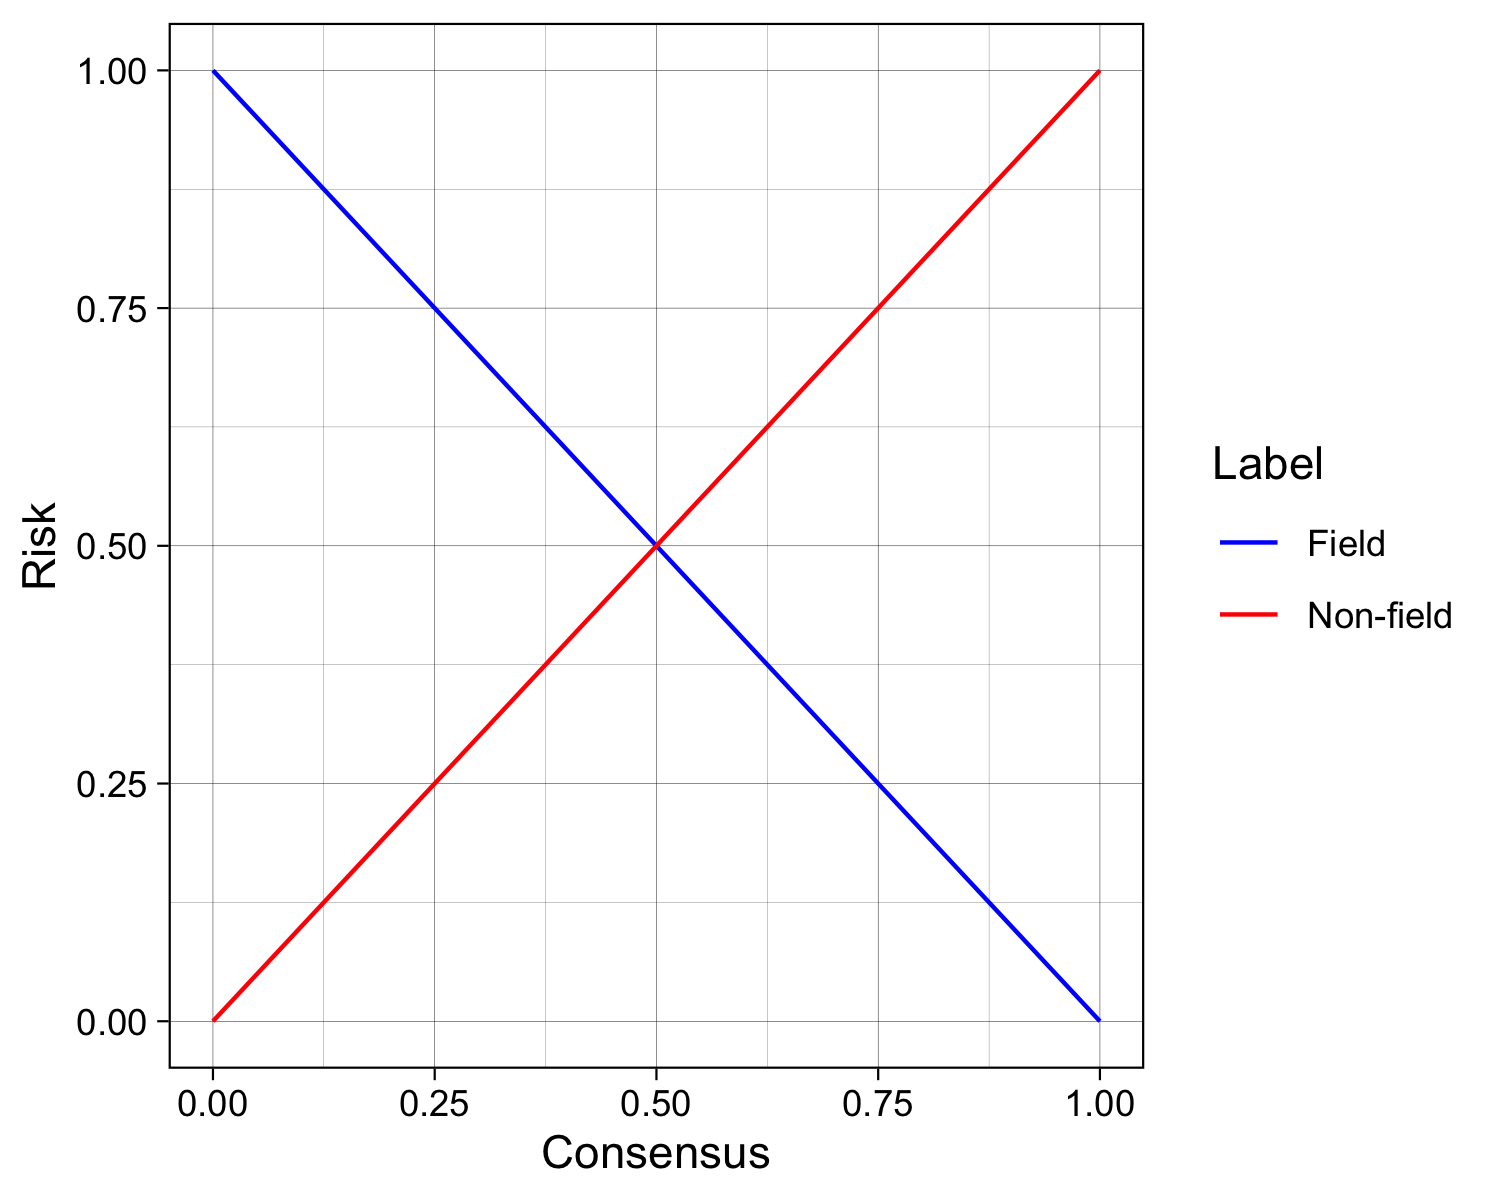
\includegraphics[width=0.7\linewidth,]{figures/si_label_risk} 

}

\caption{Bayesian risk values (Y-axis) for consensus values (X axis) ranging from 0 to 1 (0 indicates no consensus that a pixel falls into the field class, 1 means complete consensus) for field and non-field consensus labels.}\label{fig:riskcurve}
\end{figure}

Accuracy assessment and consensus label generation is performed using an
\texttt{R} package \texttt{rmapaccuracy} that is internal to the
labelling platform. The package relies on spatial data classes and
operations provided by the \texttt{sf} (Pebesma 2018) and
\texttt{raster} (Hijmans 2020) packages.

\hypertarget{example}{%
\paragraph{Example}\label{example}}

To provide an example of this approach in practice, we'll imagine two
workers A and B, each with the following histories:

\begin{longtable}[]{@{}rccr@{}}
\toprule
Worker & Prod. Acc. (Field) & Prod. Acc (no field) & Score \\
\midrule
\endhead
A & 0.80 & 0.81 & 0.75 \\
B & 0.62 & 0.61 & 0.60 \\
\bottomrule
\end{longtable}

In this scenario, worker A thinks that the given pixel falls within a
field, and worker B thinks it is not a field. First, we calculate the
weights for each worker:

\[
Weight_A = score_A * PA_A(field) = P(W_A)P(D=field|W_A) = 0.8 * 0.75 = 0.6
\]

\[
Weight_B = score_B * PA_B(field) = P(W_B)P(D=no field|W_B) = 0.61 * 0.6 = 0.366
\]

And then we plug these weights into the full equation:

\[
\mathrm{P(\theta|D)=\frac{\sum_{i=1}^{n}weight_iP(L = field|D, W_i)}{\sum_{i=1}^{n}weight_i}} = \frac{0.6 * 1 + 0.366 * 0}{0.6 + 0.366} = 0.621
\]

Since 0.621 \textgreater{} 0.5, we label the particular pixel a field.

Using equation \ref{eq:pixelrisk}, the corresponding risk associated
with this particular pixel's label is thus 0.379 (i.e., 1 - 0.621).

\hypertarget{segmentation}{%
\subsubsection{Segmentation}\label{segmentation}}

An overview of the two inputs to and outputs from the segmentation
algorithm are shown in Figure \ref{fig:segfig}.

\begin{figure}[!ht]

{\centering 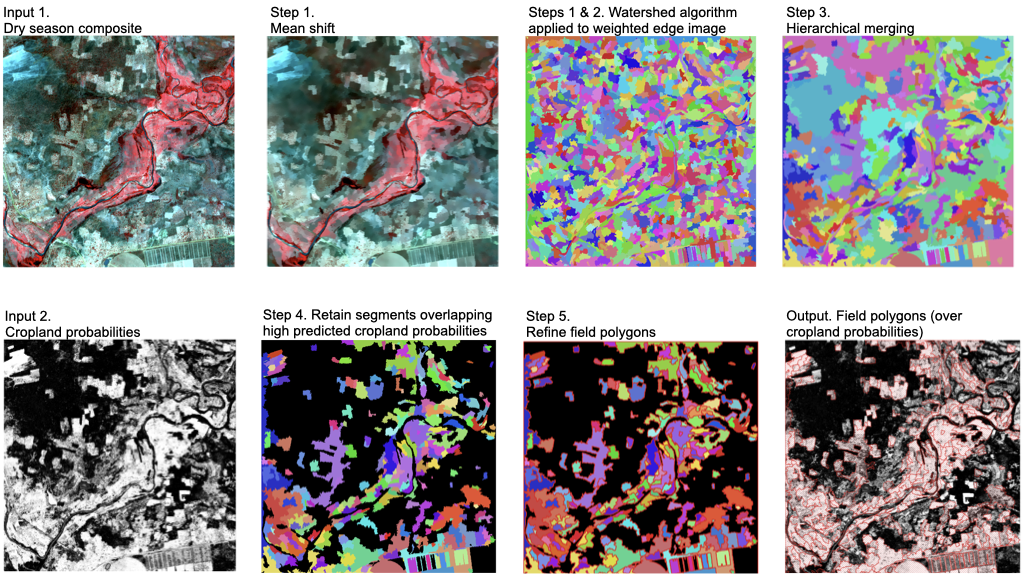
\includegraphics[width=1\linewidth,]{figures/si_segmentation_workflow} 

}

\caption{An overview of the inputs and key outputs from the five-step segmentation algorithm.}\label{fig:segfig}
\end{figure}

\hypertarget{accuracy-assessment}{%
\subsubsection{Accuracy assessment}\label{accuracy-assessment}}

We designed and implemented a map accuracy assessment protocol following
procedures summarized by Stehman and Foody (2019). This entailed the
creation of a map reference sample, which first entailed designing a
sample, and then designing how the sample response would be collected.

\hypertarget{map-reference-sample-design}{%
\paragraph{Map reference sample
design}\label{map-reference-sample-design}}

We employed a stratified design for collecting the map reference sample,
using the segmented field boundaries to define the strata for
cropland/non-cropland. To create the sample, we first extracted the
centroids for each of the sample grid cells in Ghana. We then
intersected the centroid points with the field segments, assigned a
class of 1 (cropland) where points intersected a field, and 0 where they
didn't (non-cropland). We removed from this set of points all those that
corresponded to model training, validation, or training reference sites,
and extracted a random sample from both the cropland and non-cropland
points. To determine the sample size of each, we specified a desired
confidence interval using the following formula (Stehman and Foody
2019):

\[n = \frac{z^2p(1-p)}{d^2}\]

Where p is the estimated probability (or mapped class accuracy), and d
is the size of the margin of error (1/2 the confidence interval). We
selected a d value of 0.03 and assumed that the user's accuracy of the
field class would be 0.75 and that of the non-cropland class would be
0.8, returning sample sizes of 800 and 683, respectively. The
distribution of the resulting map reference sample is shown in Figure
\ref{fig:refsample}.

\begin{figure}[!ht]

{\centering 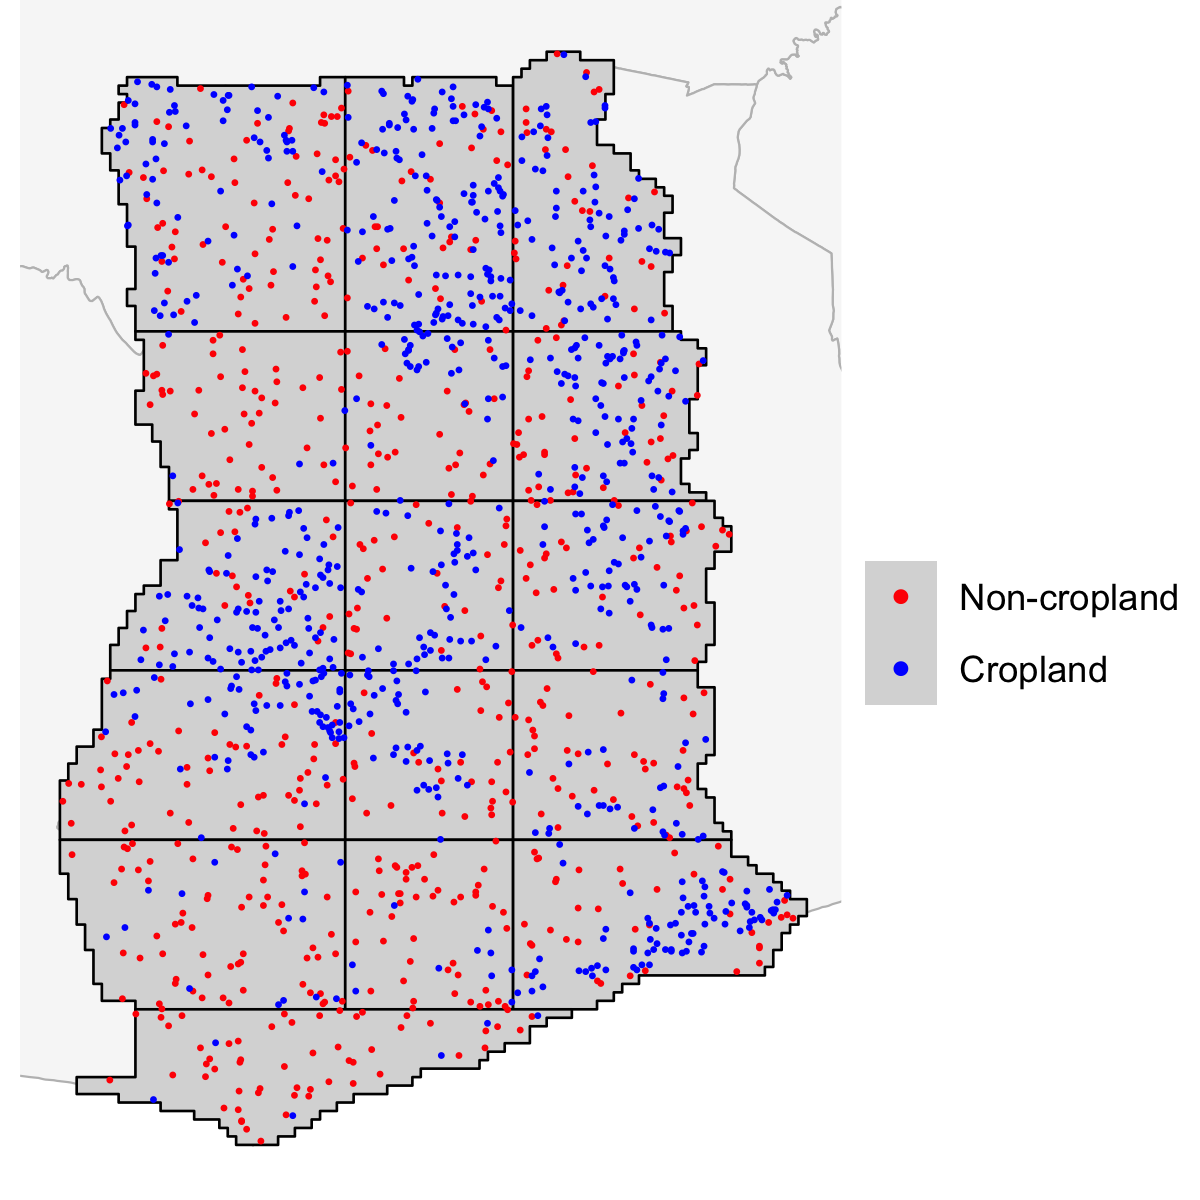
\includegraphics[width=0.8\linewidth,]{figures/si_map_reference_sample} 

}

\caption{Distribution of the selected map reference sample for the cropland and non-cropland class. Classes represent the values extracted from the map strata, rather than those assigned during the classification of the sample.}\label{fig:refsample}
\end{figure}

\hypertarget{response-design}{%
\paragraph{Response design}\label{response-design}}

We collected the map reference sample on a separate instance of the
labelling platform set up for the purpose. For the sampling unit, we
selected a rectangular polygon of \textasciitilde0.1 ha
(0.0002866\(^\circ\) resolution). This polygon was centered on the
centroid of each grid cell selected for map reference sample, and was
presented as the target grid in the labelling platform. Four classes
were established for the validation: \textbf{cropland},
\textbf{non-cropland}, \textbf{uncertain but likely cropland}, and
\textbf{uncertain but likely non-cropland}. The latter two classes were
designed to capture information related to swidden dynamics, following
the rationale that uncertainty and time since last cropping are likely
to be positively correlated. This uncertainty also captures information
about the inherent difficulty of the mapping task. Samples were
collected by visually interpreting the overlays of PlanetScope
composites, following the same interpretation protocols used by the
labelling team, with the exception that the polygons placed were square
and of 0.0002866\(^\circ\) resolution.

Two supervisors (Ye and Estes), who were not involved in collecting
training and validation labels, collected the map reference sample by
evaluating the PlanetScope composites at each site to determine its
class membership. The following set of rules were followed in collecting
the sample:

\begin{enumerate}
\def\labelenumi{\arabic{enumi}.}
\tightlist
\item
  When determining the class corresponding with the initial location of
  the target grid, if:
\end{enumerate}

\begin{itemize}
\tightlist
\item
  More than half of the target falls within what appears to be a clear
  arable crop field, then classify it as \textbf{cropland};
\item
  More than half falls in what is clearly not a field, then classify it
  as \textbf{non-cropland};
\item
  More than half falls in a location where it is harder to tell whether
  it is cropland or non-cropland, determine whether it is more likely a
  crop field or not a crop field, and then assign either
  \textbf{uncertain but likely cropland}, or \textbf{uncertain but
  likely non-cropland}.
\end{itemize}

\begin{enumerate}
\def\labelenumi{\arabic{enumi}.}
\setcounter{enumi}{1}
\tightlist
\item
  After determining the class, if:
\end{enumerate}

\begin{itemize}
\tightlist
\item
  The target polygon is contained entirely within a single clear class,
  then simply digitize a point within the center of the target box,
  assign the appropriate class label, and complete the assignment;
\item
  Digitize a square polygon exactly aligned with the initial target,
  choose the correct class label, and then move the new polygon to the
  nearest location where it can be contained entirely by the assigned
  class.
\end{itemize}

After collecting the sample, the geometries were further refined by
converting the points (sites were the target didn't have to be shifted)
to polygons with the same 0.0002866\(^\circ\) resolution, and then the
full set of map reference polygons was used to extract the classified
values from both the cropland probability and vectorized field boundary
maps. Accuracies were assessed for the entire country, and with several
zones consisting of different groupings of AOIs or
agroecozones\footnote{sourced from https://wheregeospatial.com/agro-ecological-zones-ghana/}

\hypertarget{map-reference-label-uncertainty}{%
\paragraph{Map reference label
uncertainty}\label{map-reference-label-uncertainty}}

The size of the collected validation sample was 1207, with 1036 samples
collected and interpreted by one observer (Su Ye) and 171 collected by a
second observer (Estes). To evaluate the uncertainty inherent in
defining the map reference labels, the pair mapped 23 common sites,
showing an overall level of agreement of 87\%, and a Spearman Rank
Correlation of 0.76.

Although this overlap between observers was limited, the map reference
classification scheme provided two additional measures of uncertainty,
which were classes defined as ``unsure but most likely a field'' or
``unsure but most likely not a field,'' which the reference labeller
would choose when they could not with high confidence state whether the
site was either cropland or not cropland. Of the 487 map reference
samples that were identified as cropland, 22\% fell into the lower
confidence category, as did 11.5\% of the 720 non-cropland samples.
Across both classes, the reference labellers had lower confidence in
15.7 of sites labelled.

\hypertarget{accuracy-assessment-zones}{%
\paragraph{Accuracy assessment zones}\label{accuracy-assessment-zones}}

The zones used to assess regional variation in map accuracy are
illustrated in Figure \ref{fig:aoizones}.

\begin{figure}[!ht]

{\centering 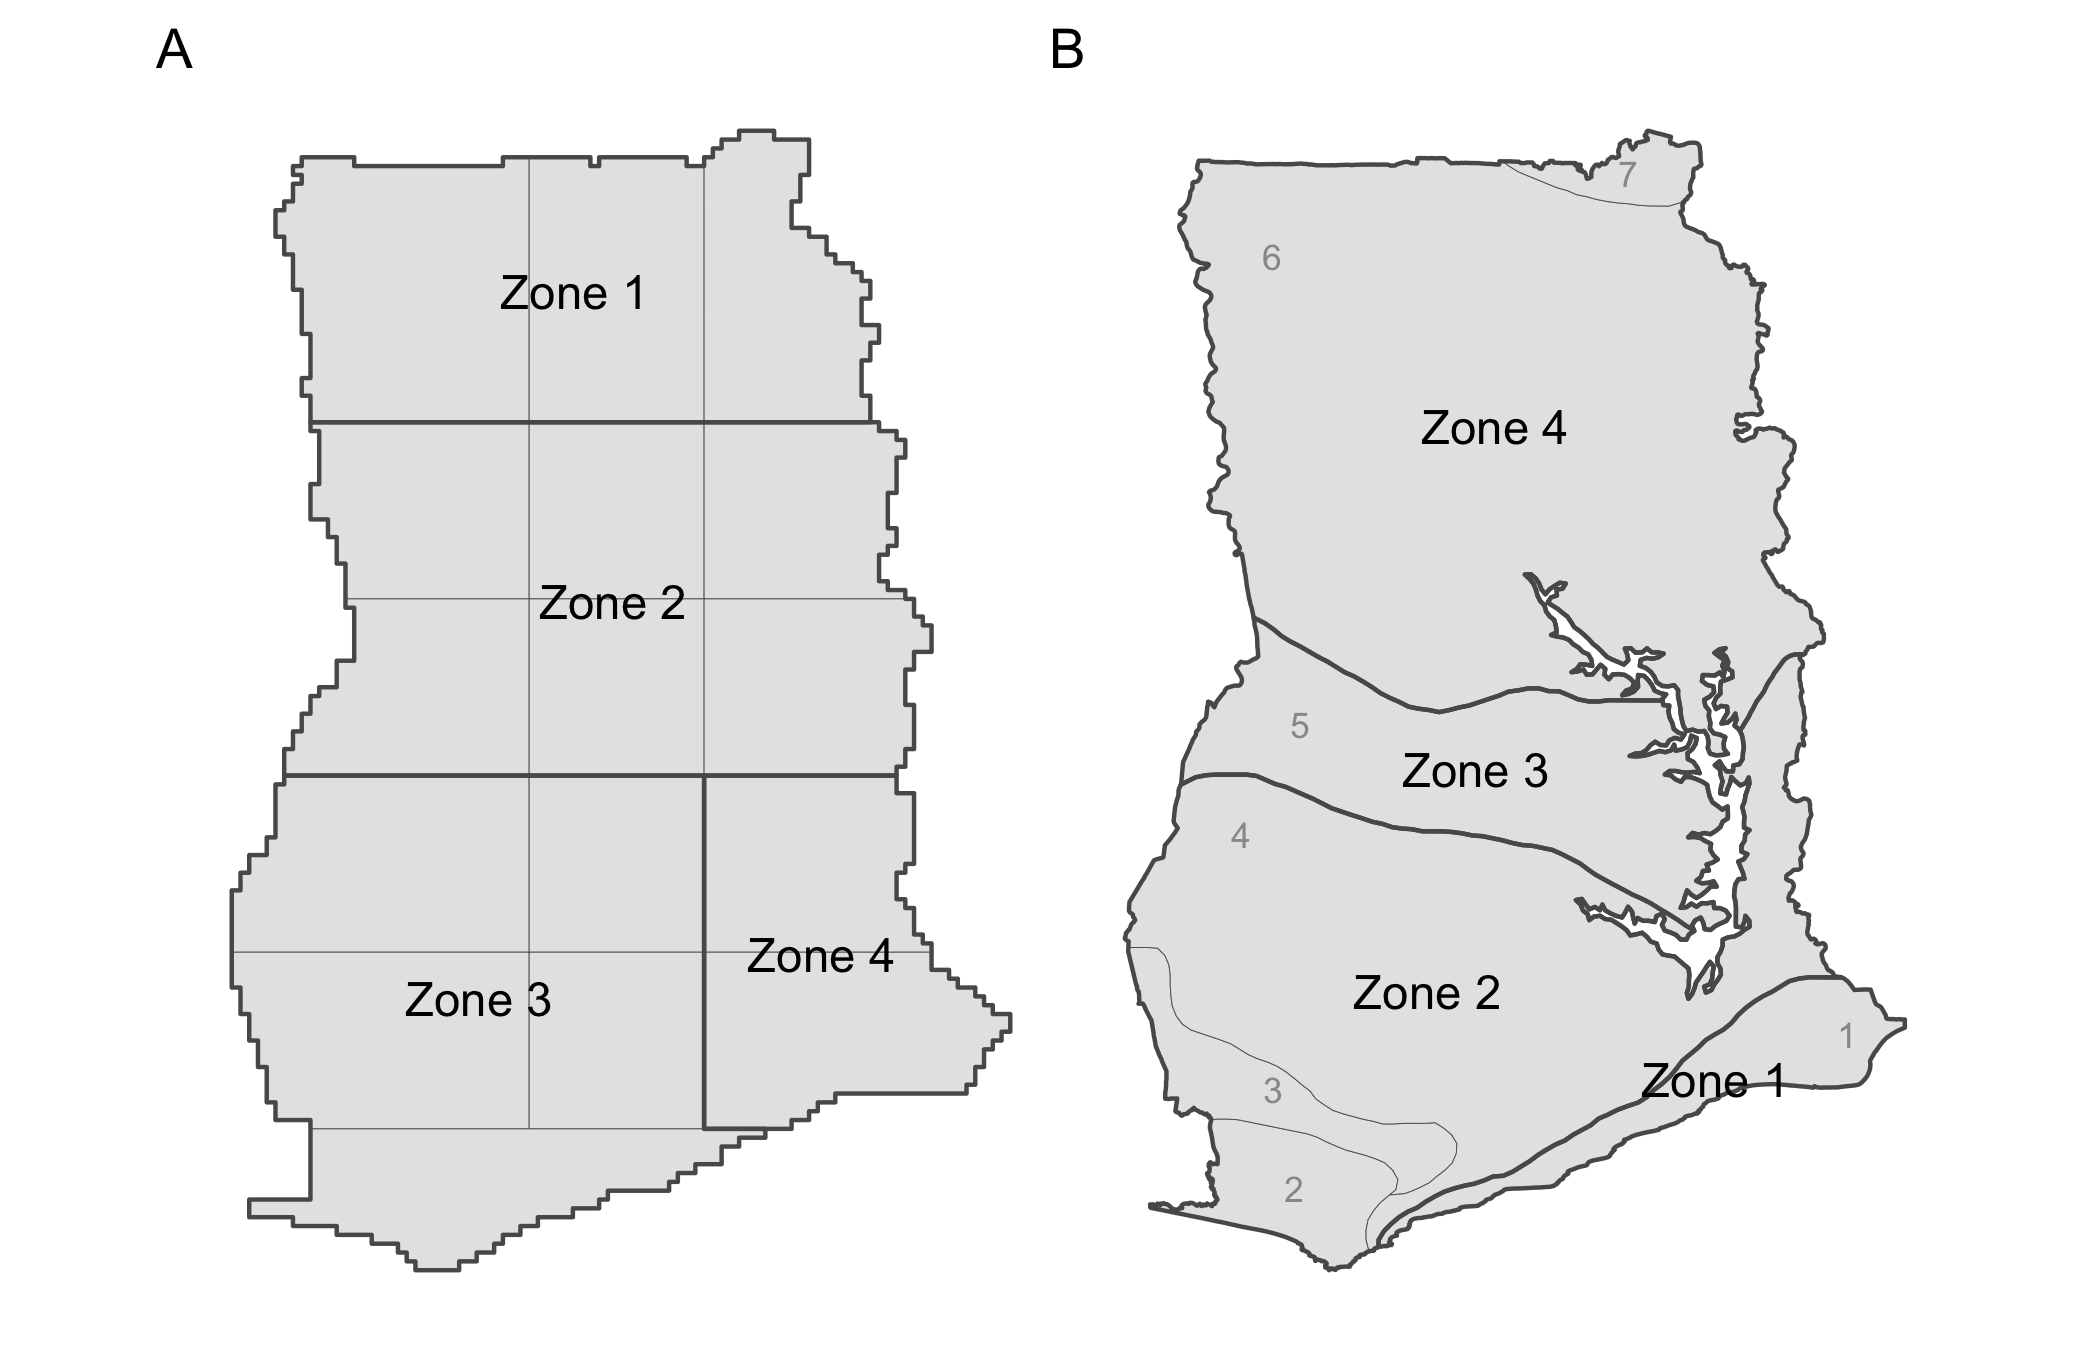
\includegraphics[width=0.9\linewidth,]{figures/si_aoi_zones} 

}

\caption{Four zones used to combine the A) AOIs and B) agroecozones (B), in order to assess sub-national mapping accuracy. In B, the ID number of Ghana's individual agroecozones is shown in grey: 1 = Coastal savanna; 2 = Wet evergreen; 3 = Moist evergreen; 4 = Deciduous forest; 5 = Transitional zone; 6 = Guinea savanna; 7 = Sudan savanna; 8 (not shown) = Volta Lake.}\label{fig:aoizones}
\end{figure}

\hypertarget{supplemental-results}{%
\section{Supplemental Results}\label{supplemental-results}}

\hypertarget{image-catalog-and-quality}{%
\subsection{Image catalog and quality}\label{image-catalog-and-quality}}

The total number of PlanetScope images available for download from the
Planet API (PlanetTeam 2018) per tile for each of the two major seasons
is shown in Figure \ref{fig:imagedensity}.

\begin{figure}[!ht]

{\centering 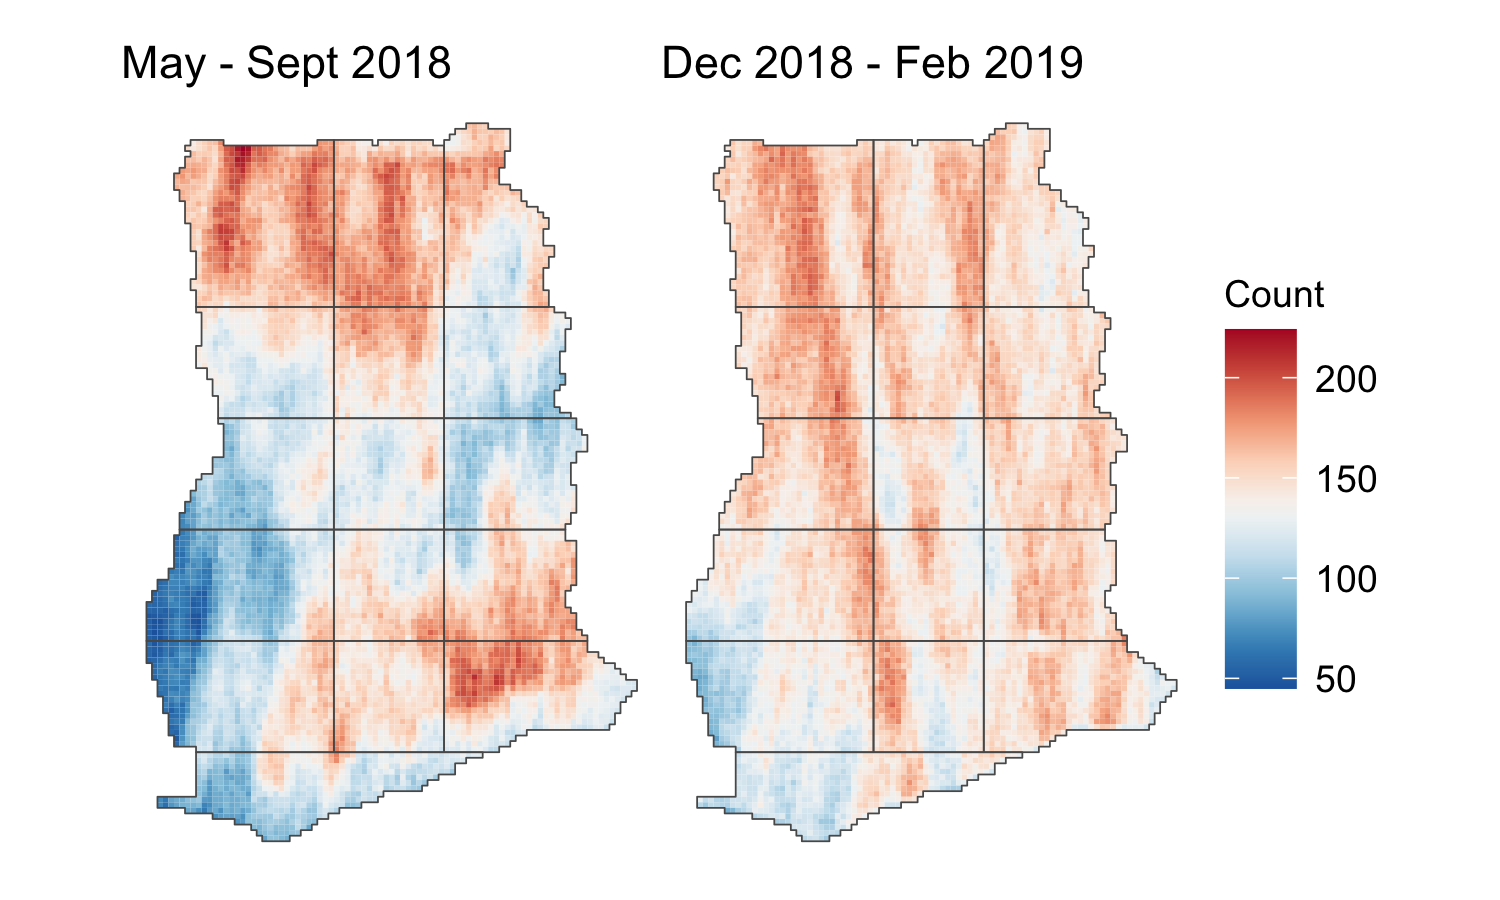
\includegraphics[width=0.9\linewidth,]{figures/si_planet_coverage} 

}

\caption{The density of images available through the Planet API for the five month growing season in 2018 and the subsequent three month dry season (excluding the month of November), shown in relation to the AOI boundaries.}\label{fig:imagedensity}
\end{figure}

The image quality assessment was conducted by two separate observers (L.
Song and Q. Zhang). Each observer assessed the composites for each
season at all 50 of the randomly selected tiles (see main text)
following the defined criteria (Table \ref{tab:imqcriteria}). To
calculate the score for a given tile for each season, we summed the
ranking across the four categories for each observer, rescaled the
values, and then calculated the mean tile score across both observers by
season. The mean difference between the two observers was -0.057 (sd =
0.081) and the mean absolute difference was 0.063 (sd = 0.076), thus one
observer scored tiles about 6 percent lower than the other observer, on
average.

\hypertarget{mapping-cropland-probabilities-with-active-learning}{%
\subsection{Mapping cropland probabilities with active
learning}\label{mapping-cropland-probabilities-with-active-learning}}

The number of active learning iterations per AOI was three, for all but
four AOIs. AOIs 10 and 14 stopped after one and two iterations,
respectively, as they started with high initial validation accuracies
(\textgreater83\%) and showed little subsequent improvement. The models
for these two AOIs were thus trained with 600 - 700 labels. AOI 15 was
run for 4 iterations (900 samples), while AOI 3 underwent a second
active learning cycle because the model produced during the first cycle
was inaccurate (see next section). In this second run, 300 initial
training sites randomly selected within the AOI were used, followed by 2
subsequent active learning iterations, resulting in a training sample of
500.

\hypertarget{labelling}{%
\subsubsection{Labelling}\label{labelling}}

The locations of training, training reference, and validation points are
shown in Figure \ref{fig:trainval}. In AOI 3, the initial active
learning cycle resulted in low accuracy because the northern part of the
AOI shows low contrast between fields and the surrounding vegetation in
the dry season. Training the model with the initial 500 samples resulted
in large commission errors in this part of the AOI, thus we ran a second
active learning cycle that began with an inital random draw of 300
training sites confined to this AOI (blue points in Figure
\ref{fig:trainval}A).

\begin{figure}[!ht]

{\centering 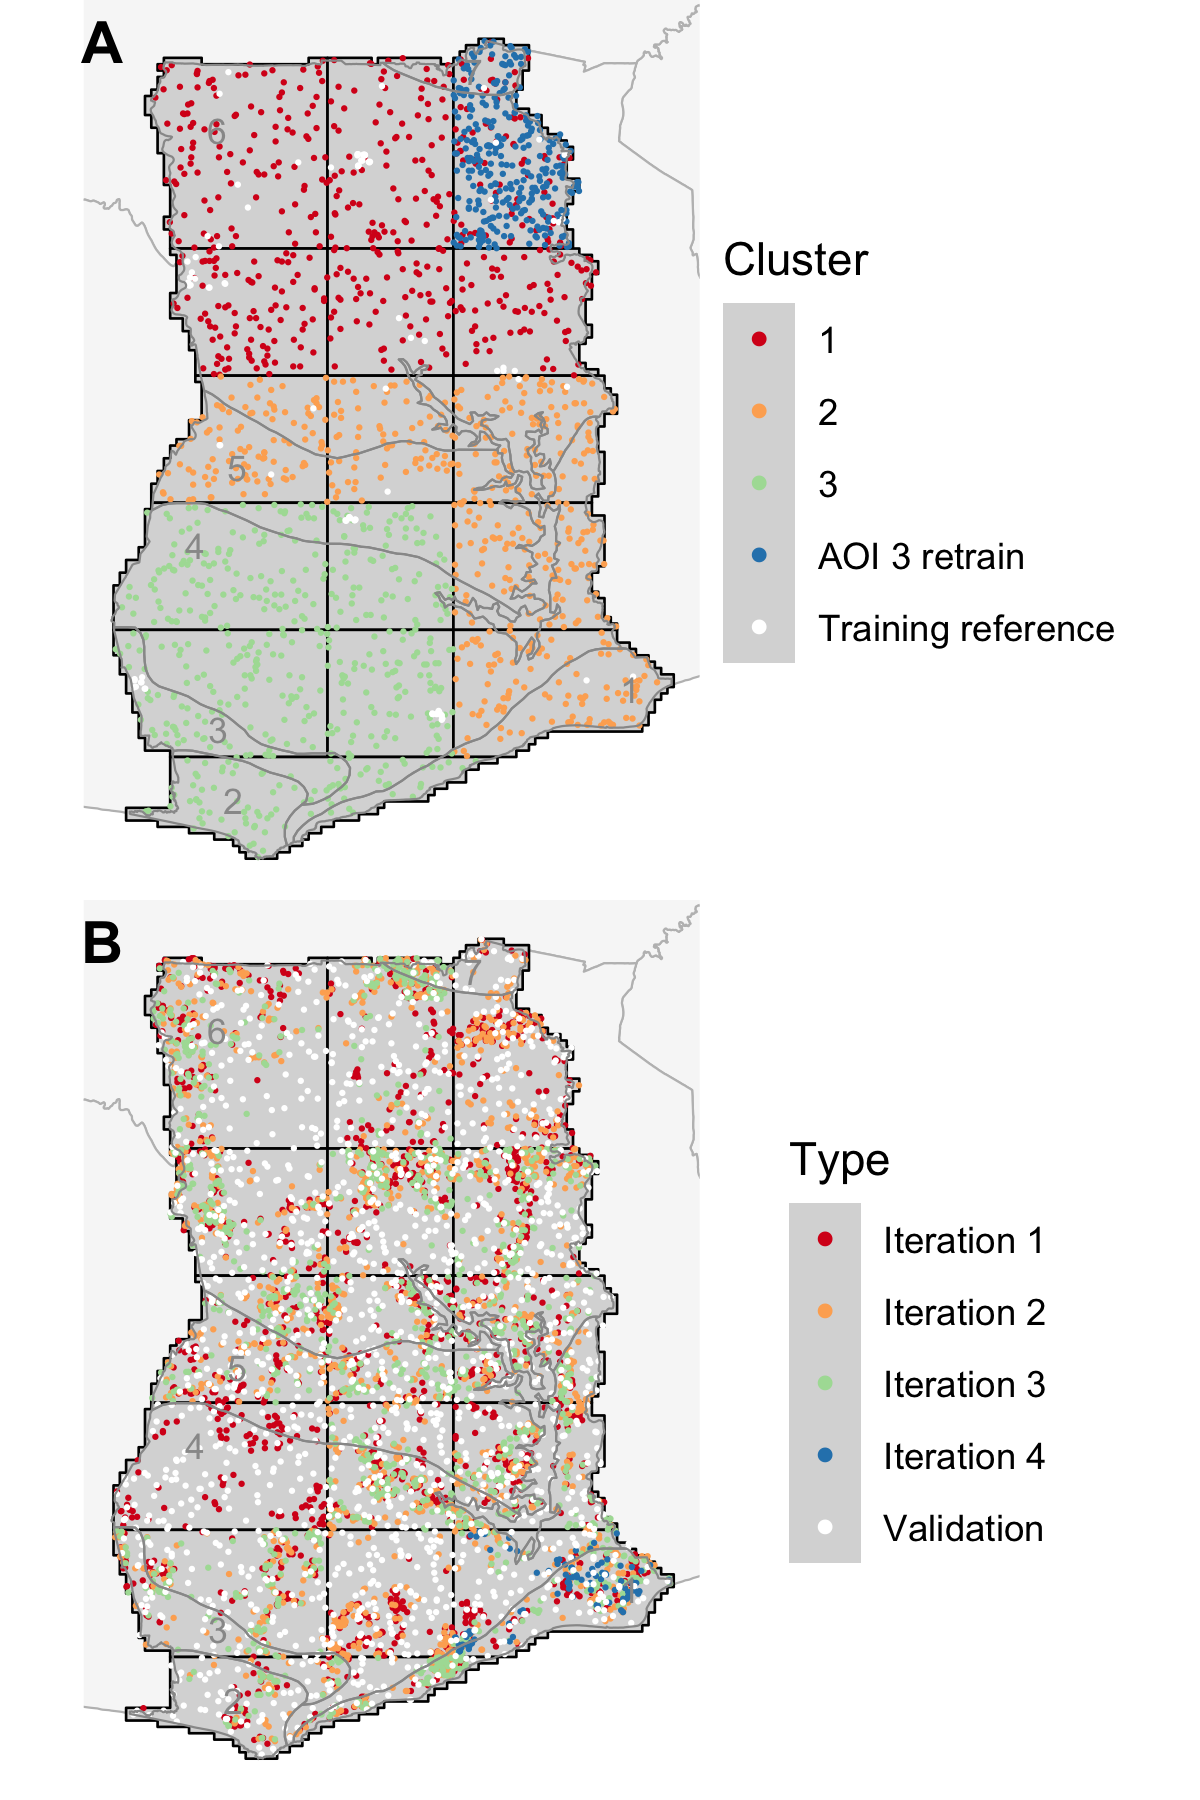
\includegraphics[width=0.7\linewidth,]{figures/si_training_validation_pts} 

}

\caption{The distribution of A) initial randomly selected training sites, including 300 points selected to initialize a second run for retrain AOI 3, and the locations of training reference sites, and B) validation points and training sites selected during each active learning iteration. Grey background lines and show the boundaries and ID number of Ghana's agroecozones: 1 = Coastal savanna; 2 = Wet evergreen; 3 = Moist evergreen; 4 = Deciduous forest; 5 = Transitional zone; 6 = Guinea savanna; 7 = Sudan savanna; 8 (not shown) = Volta Lake.}\label{fig:trainval}
\end{figure}

The distribution of training and validation sample collection effort was
divided across 20 labellers, with a core group of 13 who completed more
than 1,000 assignment each (Figure \ref{fig:assignmentcount}). As each
training/validation task was undertaken by 4 separate labellers, 34,014
sets of labels were made. Each labeller digitized an average of 2,001
training/validation assignments.

\begin{figure}[!ht]

{\centering 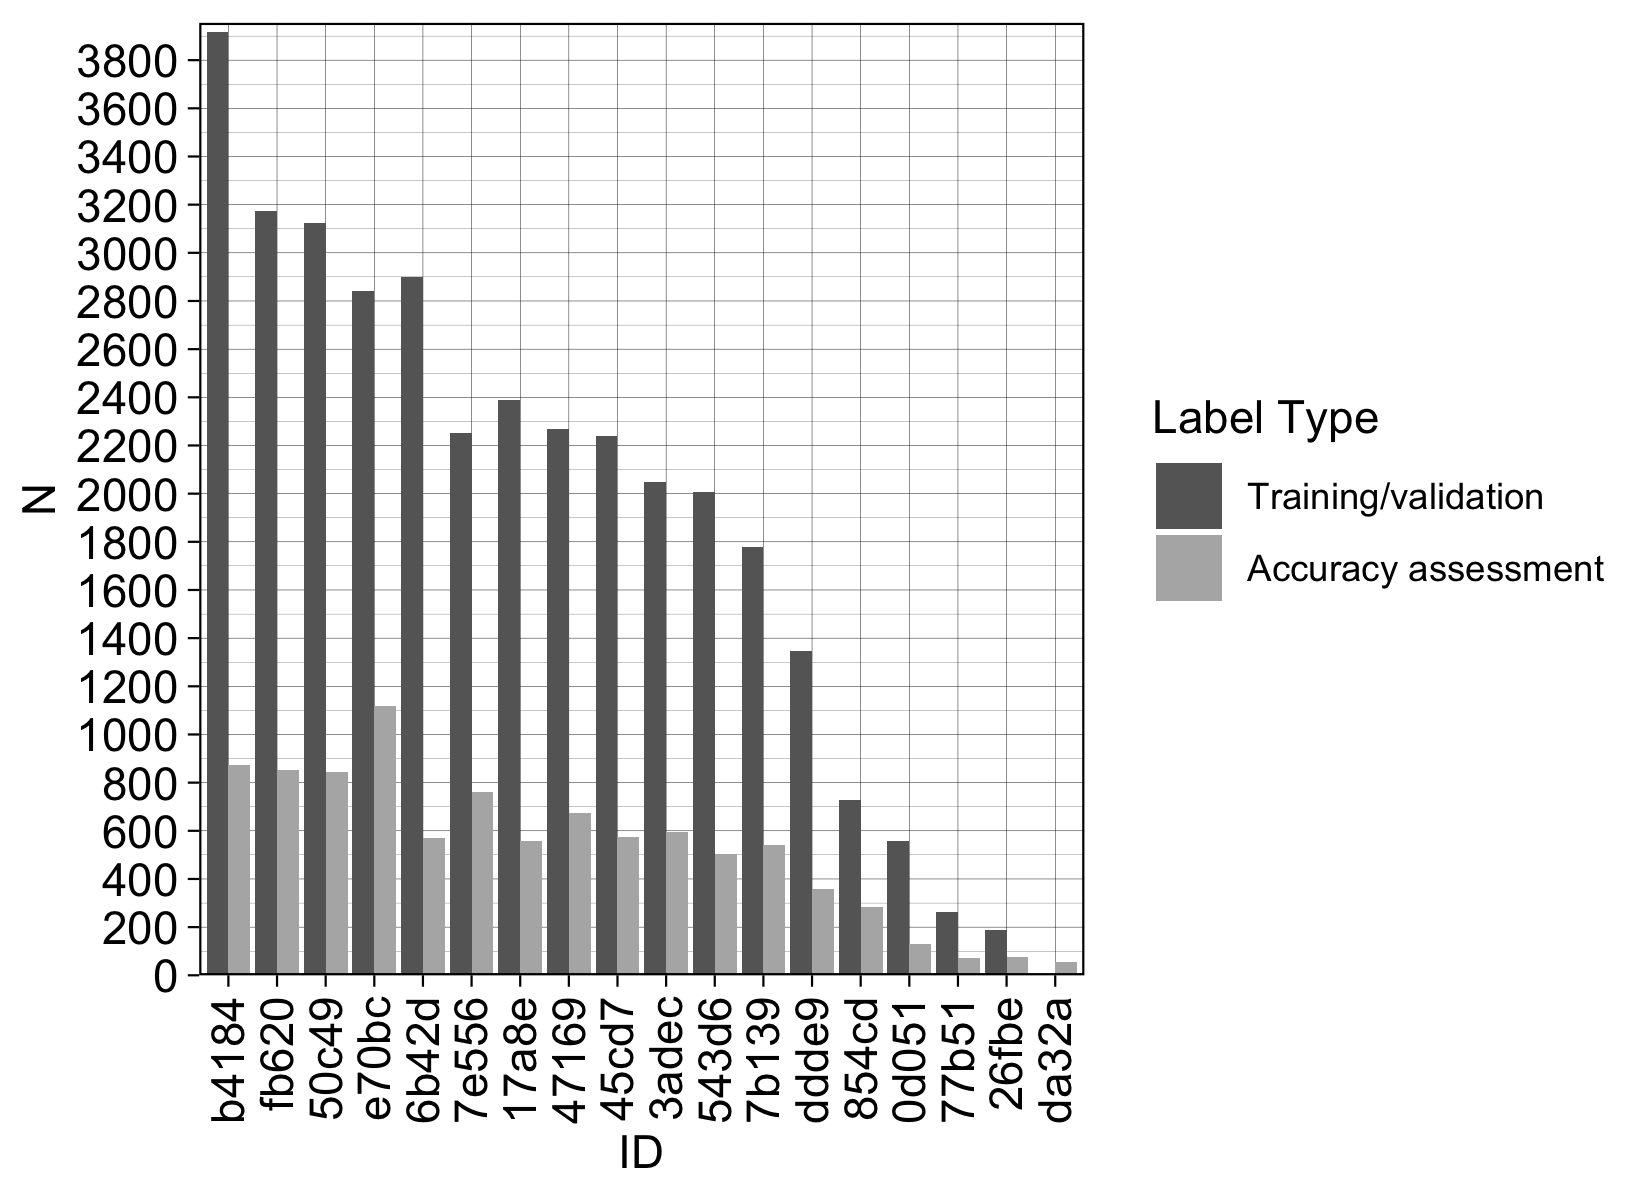
\includegraphics[width=0.8\linewidth,]{figures/si_training_n} 

}

\caption{The A) number of training/validation and accuracy assessment assignments completed by each labeller, and B) the distributions of quality scores at training reference sites for each labeller (means indicated by X in boxplots). Labellers' identities are anonymized.}\label{fig:assignmentcount}
\end{figure}

These results include those from re-labelling the initial training in
Cluster 2 (AOIs 7-9, 12, 15). This was done because we discovered a
small spatial offset in the original image composites, which we
corrected by reprocessing the images. We replaced the image overlays in
the instances for this Cluster (Figure \ref{fig:trainval}A), and the
labelling team mapped these sites a second time during the production
run in late 2019. The reprocessed labels were used to initially train
the model for AOIs 9, 12, and 15.

\hypertarget{model-performance}{%
\subsubsection{Model performance}\label{model-performance}}

The differences in accuracy, AUC, and F1 between the active learning
process and the random retraining at each iteration for AOIs 1, 8, and
15 (Figure \ref{fig:randomvactive}). Small differences due to random
variations in the RandomForest models are the reason for the non-zero
differences at iteration 0, when both models were trained with the same
level set.

\begin{figure}[!ht]

{\centering 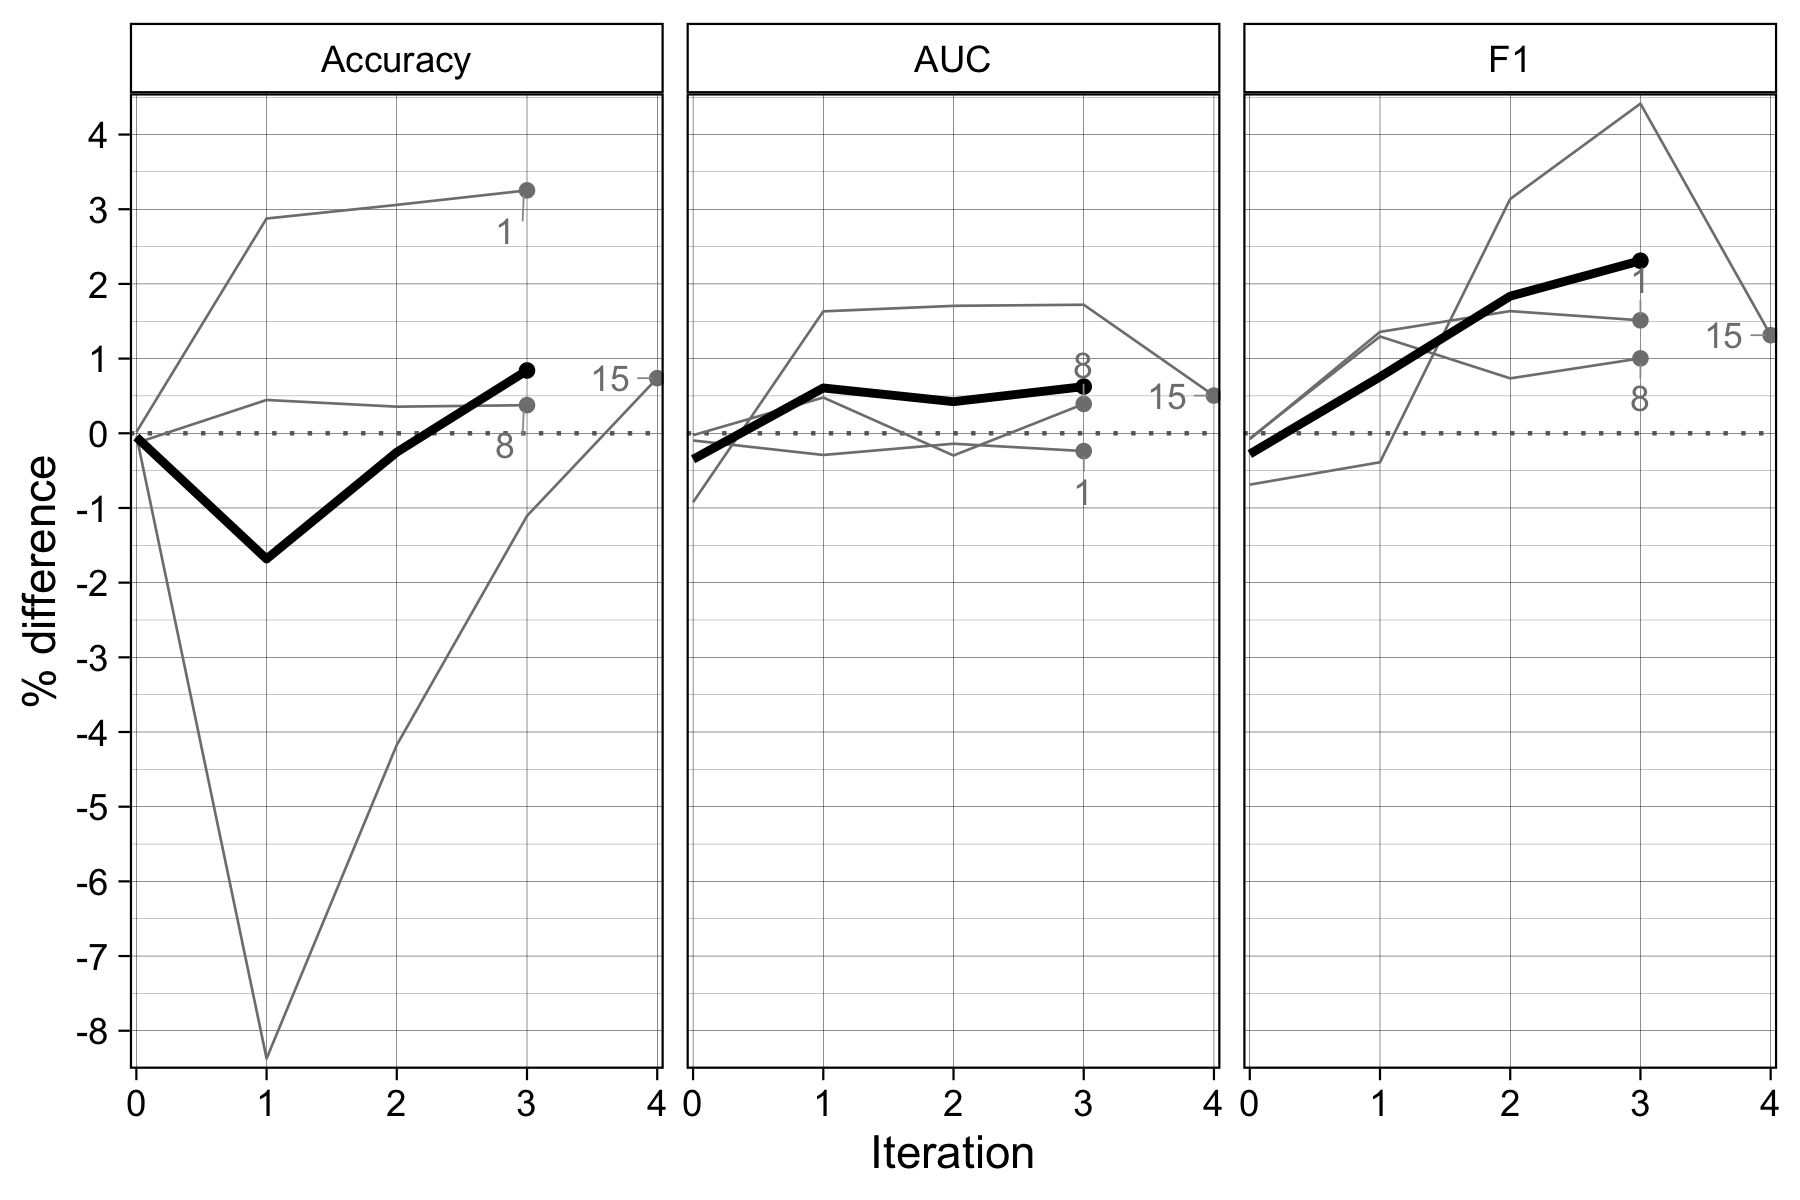
\includegraphics[width=0.9\linewidth,]{figures/si_random_vs_active} 

}

\caption{The percent difference in performance metrics per iteration for AOIs 1, 8, and 15 (grey lines with numbers indicating AOI; the black line indicates average difference across the three AOIs) when comparing models trained using active learning versus those trained using randomly selected sites. Postive percentages indicate superior performance by active learning, negative percentages the inverse.}\label{fig:randomvactive}
\end{figure}

The lower accuracy of actively versus randomly trained models in earlier
iterations was caused by results at AOI 15, where active learning
accuracy was 8.37 percent lower than random training after iteration 1
(see Figure \ref{fig:randomvactive}). In comparison, iteration 1 active
learning accuracies were 2.88 and 0.45 percent higher than random
training for AOIs 1 and 8, respectively. Accuracy under active learning
for AOI 15 exceeded randomized training after 4 iterations.

\hypertarget{the-impact-of-training-data-error}{%
\subsubsection{The impact of training data
error}\label{the-impact-of-training-data-error}}

Two measures of label quality, average quality score per labeller and
the Bayesian Risk of labels, were calculated to provide proxy measures
of label error. Labeller quality was scored 9,389 times against 98
unique training reference sites, with each labeller assessed an average
of 552 times at a rate of 1 training reference site for every 3.62
training site mapped. The mean of each labeller's average accuracy score
was 0.71 (range 0.6 to 0.85; Figure \ref{fig:labelqual}).

\begin{figure}[!ht]

{\centering 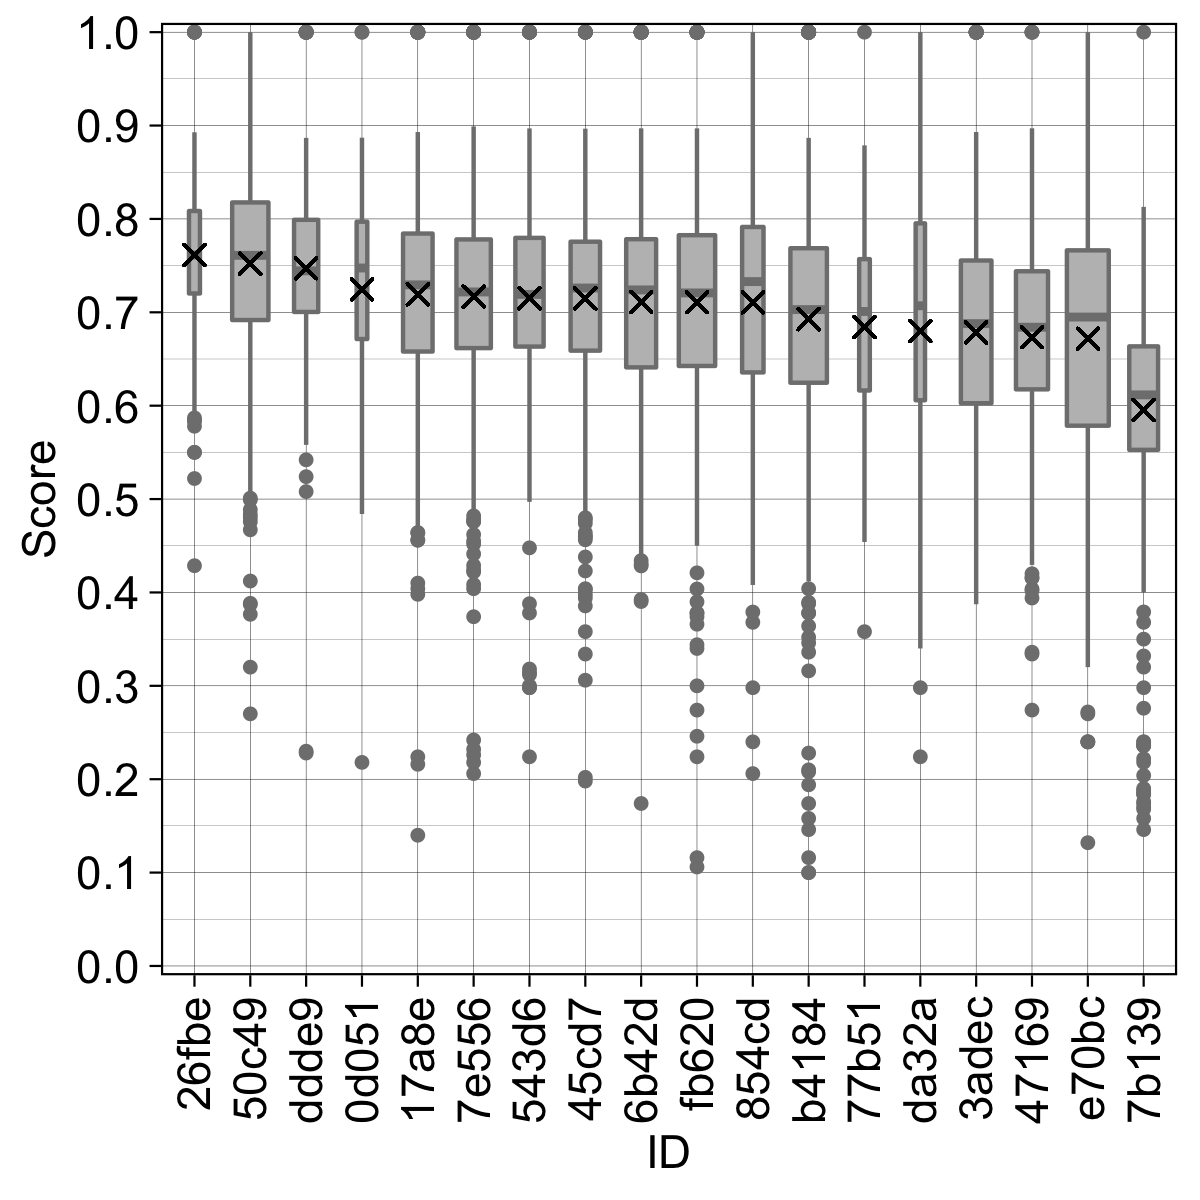
\includegraphics[width=0.7\linewidth,]{figures/si_label_quality} 

}

\caption{Boxplots showing the distributions of quality scores from the accuracy assessment assignments undertaken by each labeller (means indicated by X in boxplots). Labellers' identities are anonymized.}\label{fig:labelqual}
\end{figure}

The average Bayesian Risk of each training and validation site is shown
in Figure \ref{fig:labelrisk}, and the distribution of risk values per
AOI and the initial training clusters in Figure \ref{fig:labelriskhist}.
The three initial clusters include the second mapping of Cluster 2
(Figure \ref{fig:trainval}A).

\begin{figure}[!ht]

{\centering 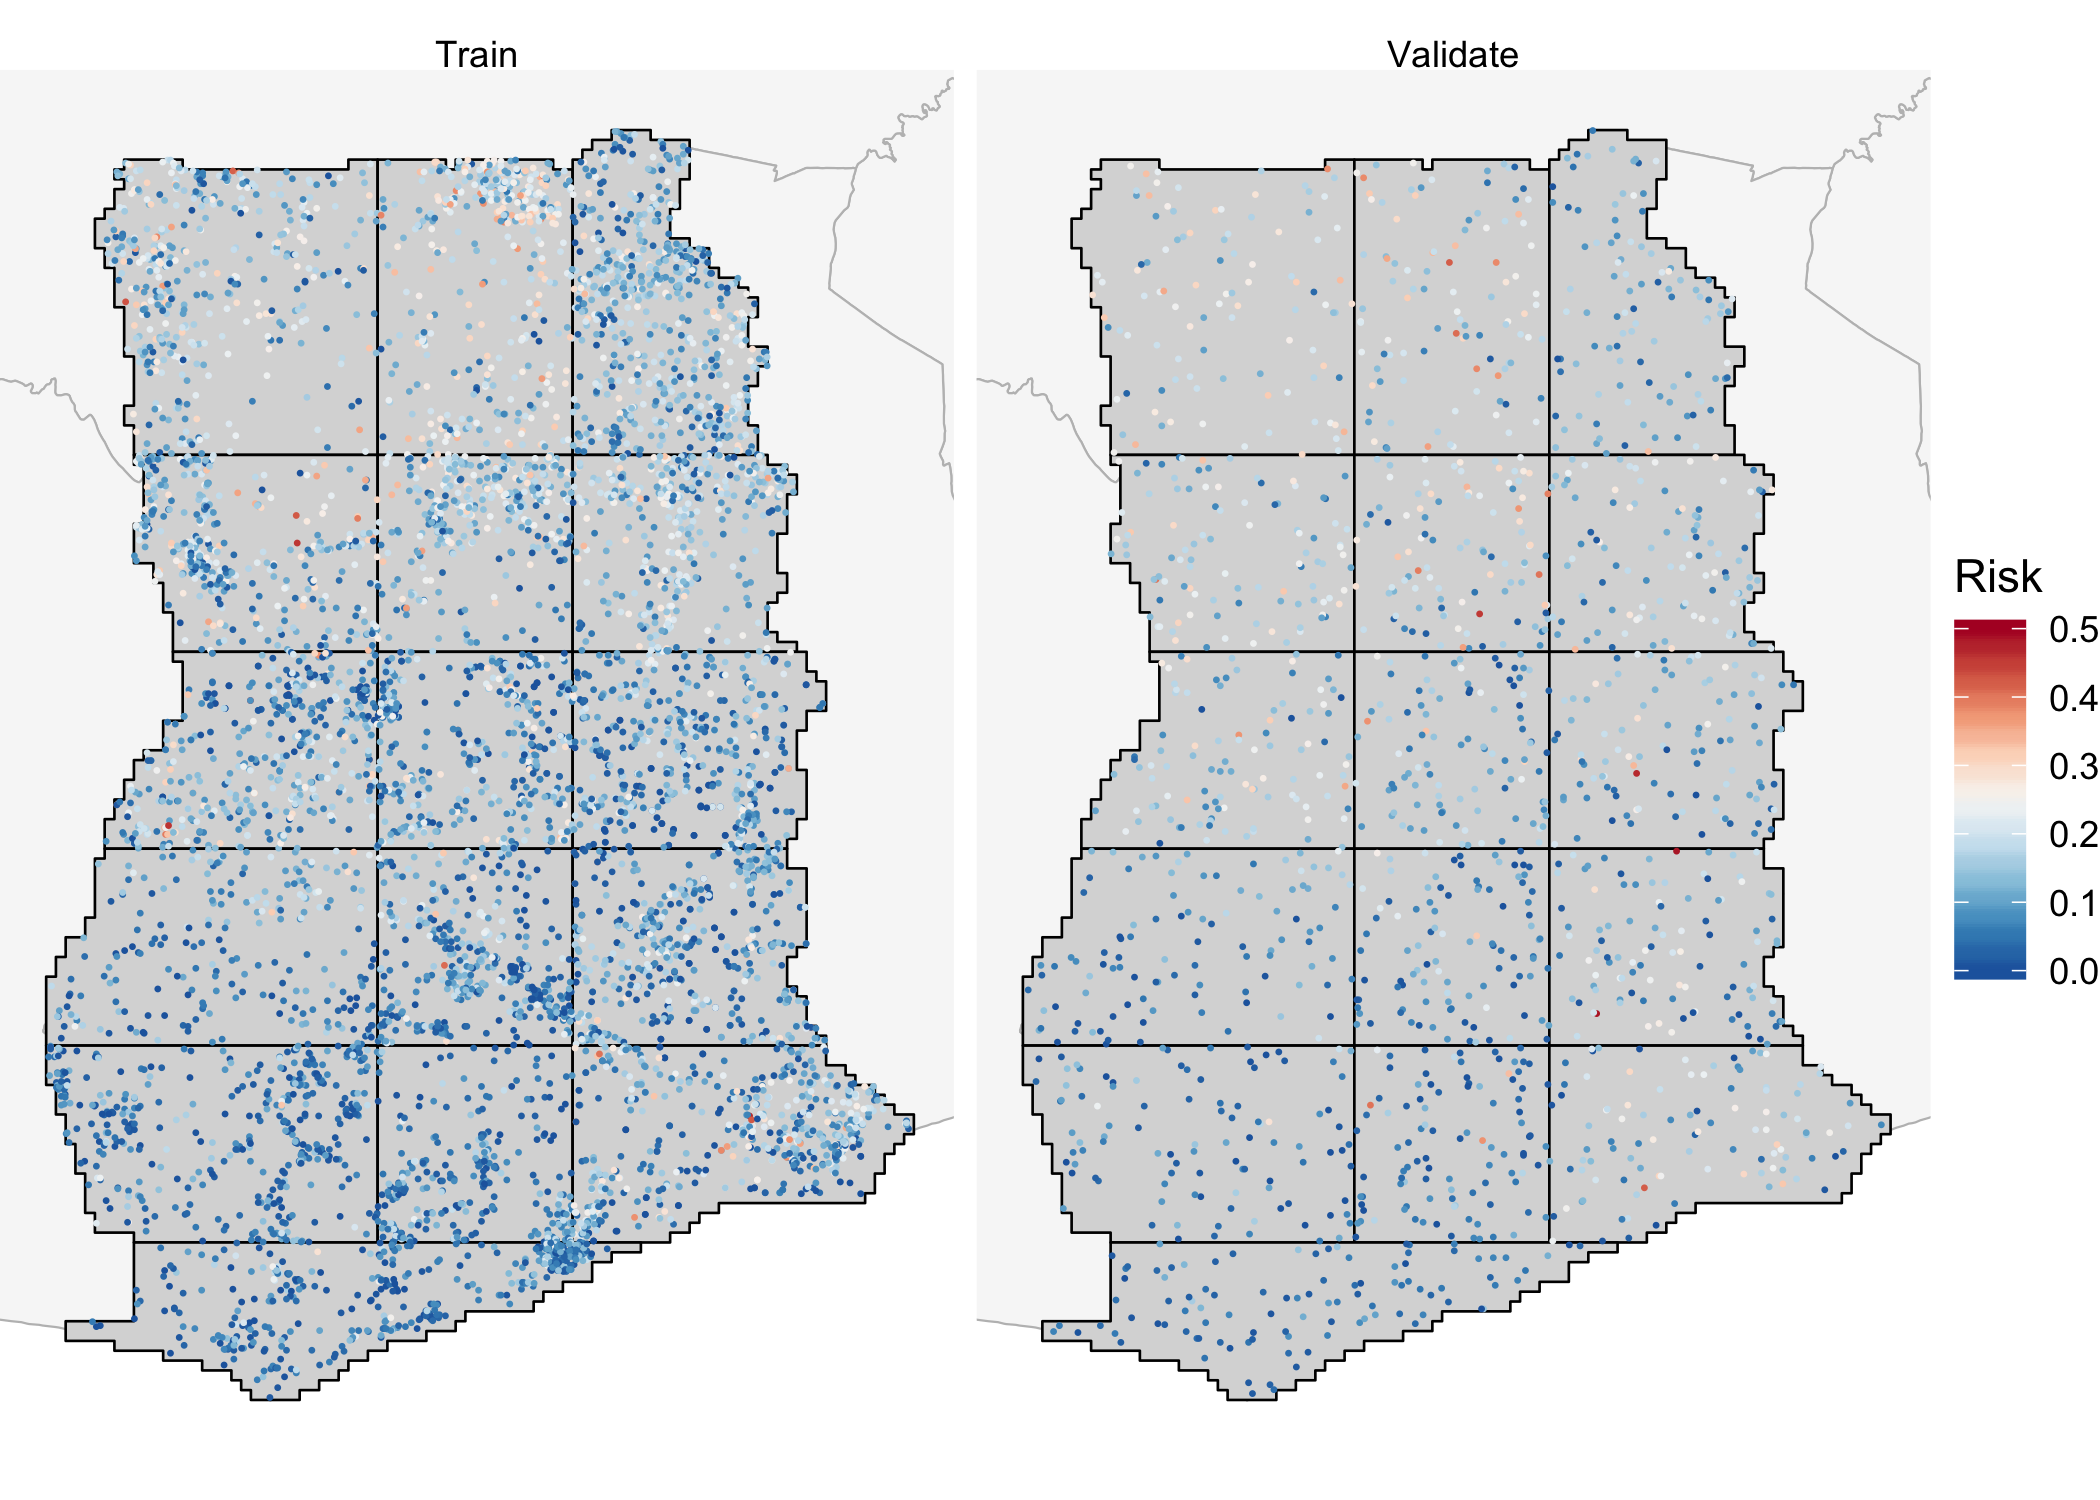
\includegraphics[width=0.8\linewidth,]{figures/si_label_risk_map} 

}

\caption{The average Bayes Risk of each training and validation site in Ghana.}\label{fig:labelrisk}
\end{figure}

\begin{figure}[!ht]

{\centering 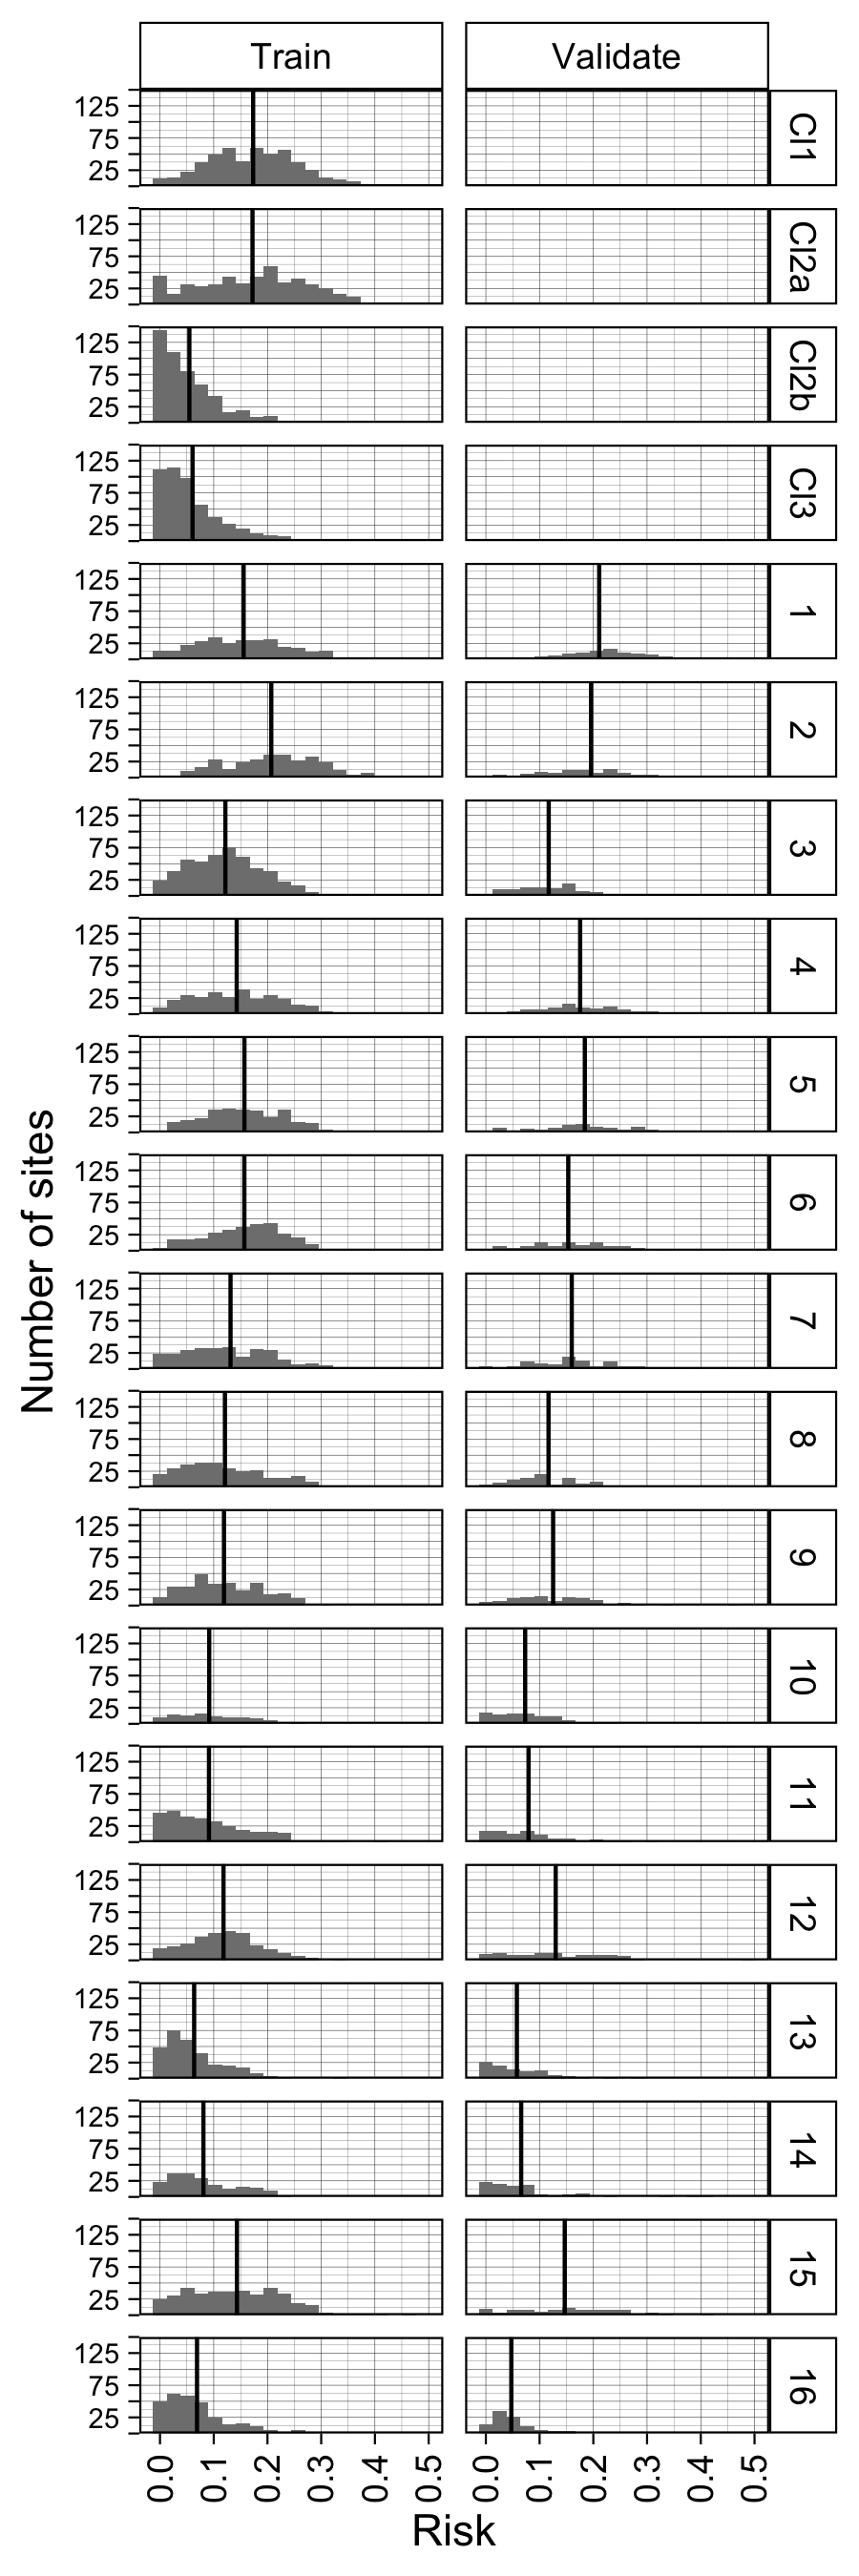
\includegraphics[width=0.4\linewidth,]{figures/si_label_risk_hists} 

}

\caption{The distribution of Bayesian Risk values for training (left column) and validation (right column) sites in each AOI, with the average value indicated by vertical lines. The first three rows (panel titles beginning with 'Cl') indicate distributions of Bayes Risk in the initial training clusters, including the first ('Cl2a') and second ('Cl2b') mappings of Cluster 2.}\label{fig:labelriskhist}
\end{figure}

The average Bayesian risk was 0.122 for training labels and 0.127 for
validation labels. Risk was highest in the northern AOIs (AOIs 1-6;
Figures \ref{fig:labelrisk}-\ref{fig:labelriskhist}), falling between
0.157 for training and 0.173 for validation labels, and lowest in the
southwestern AOIs (AOIs 10, 11, 13, 14, 16; training risk = 0.079;
validation risk = 0.065). Label risk in the central-southeastern AOIs
(AOIs 7-9, 12, 15) was slightly lower (training = 0.127; validation =
0.136) than in the north. Labeller experience also appeared to reduce
risk, which we observed during a relabelling of the 500 initial random
site in this cluster; the mean risk of the updated labels was 0.055,
compared to 0.172 for original labels.

Probability images resulting from Random Forests models trained with
labels generated under three different labeling strategies are
illustrated in Figure \ref{fig:labelstrategy}. These included consensus
labels, and those individual labels that were likely to be the most and
least accurate for each training site. Label accuracy was based on the
mean score of each labeller against the training reference sites (Figure
\ref{fig:labelqual}), as assessed when labelling a given AOI. These
images were created for a single tile in AOI 1.

\begin{figure}[!ht]

{\centering 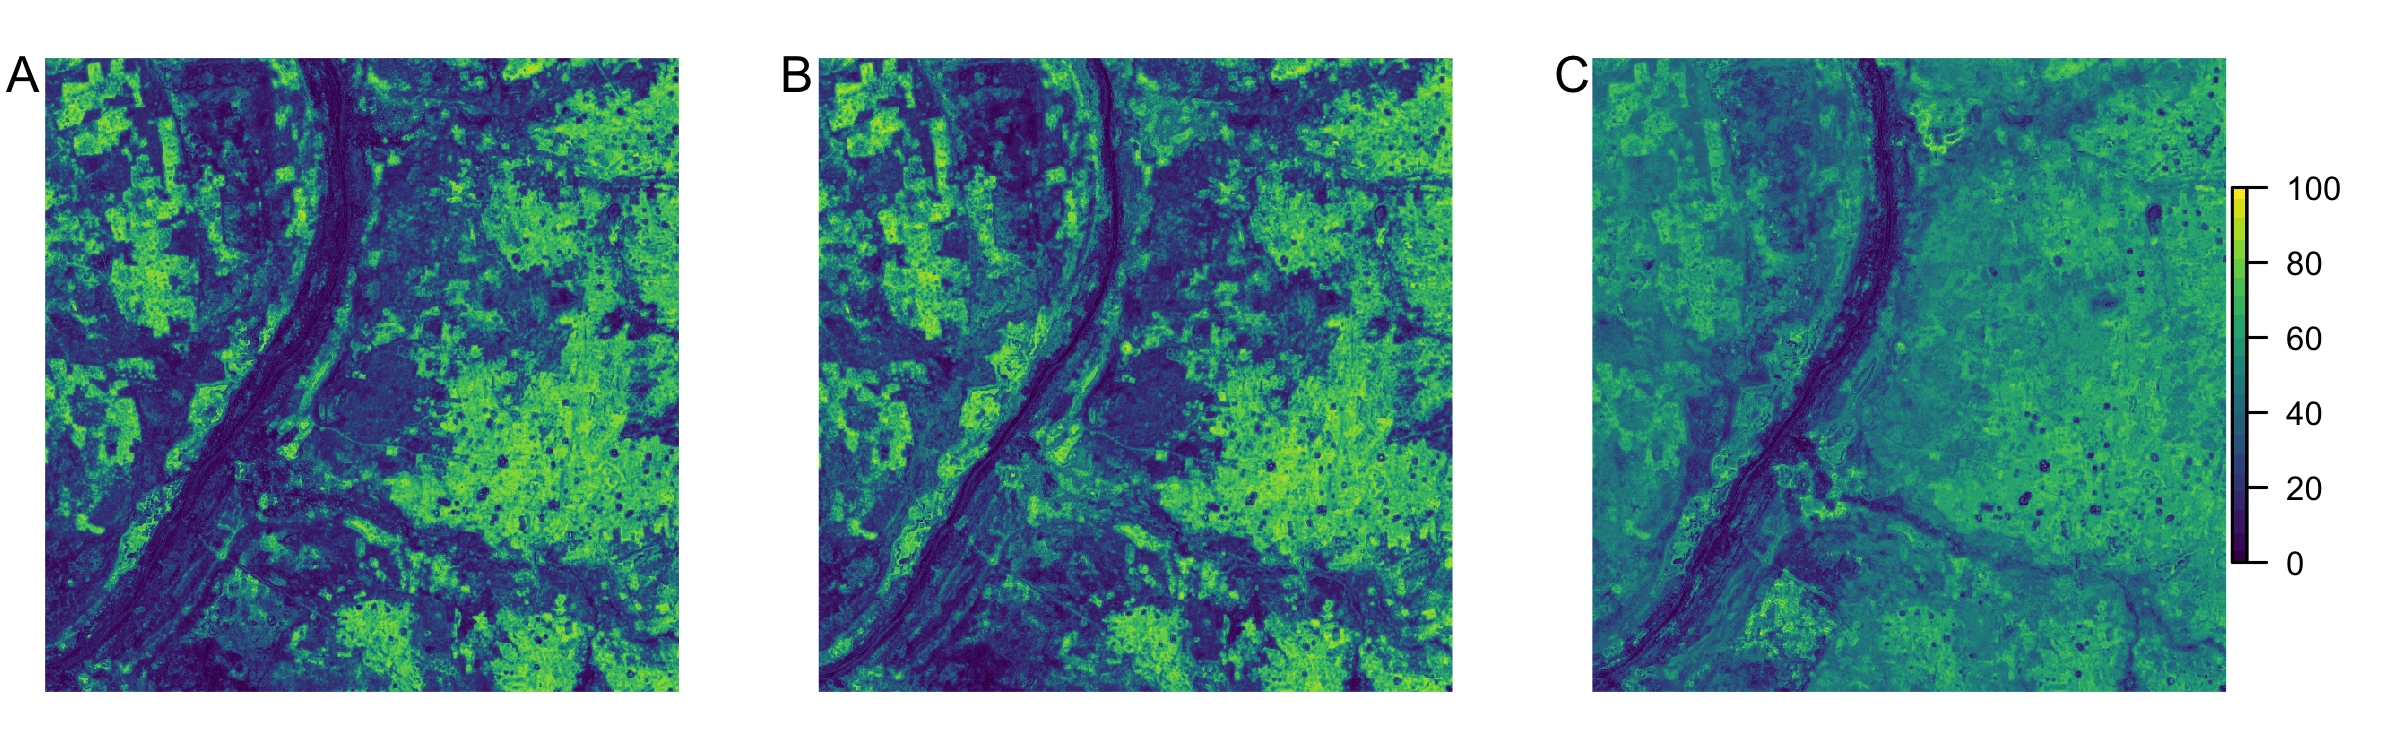
\includegraphics[width=1\linewidth,]{figures/si_label_strategy_probs} 

}

\caption{Cropland probability images produced by Random Forests models trained with A) consensus labels, B) the most accurate individual labels, and C) the least accurate individual labels.}\label{fig:labelstrategy}
\end{figure}

The association between the average label risk per AOI and several model
performance metrics, assessed using Spearman Rank Correlation, is shown
in Table \ref{tab:labelrisk_v_metrics}.

\begin{table}[!h]

\caption{\label{tab:labelrisk_v_metrics}Spearman's Rank correlation between the average label risk per AOI and a variety of model performance metrics.}
\centering
\begin{tabu} to \linewidth {>{\raggedright}X>{\raggedleft}X>{\raggedleft}X>{\raggedleft}X>{\raggedleft}X>{\raggedleft}X>{\raggedleft}X}
\toprule
  & Accuracy & AUC & F1 & Precision & Recall & FPR\\
\midrule
r & -0.824 & -0.568 & 0.456 & 0.629 & 0.206 & 0.688\\
\bottomrule
\end{tabu}
\end{table}

\hypertarget{map-accuracy}{%
\subsection{Map accuracy}\label{map-accuracy}}

\hypertarget{categorical-accuracy}{%
\subsubsection{Categorical accuracy}\label{categorical-accuracy}}

In addition to the map accuracies and area estimates calculated per AOI
zone (reported in main text; see Figure \ref{fig:aoizones}A), the
accuracies were also assessed within several different groupings of
agroecozones (Figures \ref{fig:aoizones}B and Table
\ref{tab:aezaccuracy}).

\begin{table}
\caption{Map accuracies and adjusted area estimates for the ~3 m pixel-wise classifications (based on RandomForest predictions). Results are provided for four different groupings of Ghana's 8 agroecozones zones (Zone 1 = Coastal savanna; Zone 2 = Wet evergreen, Moist evergreen, and Deciduous forest; Zone 3 = Transitional zone; Zone 4 = Guinea savanna and Sudan savanna) plus the entire country. The error matrix (with reference values in columns) provides the areal percentage for each cell, and the producer's (P), user's (U), and overall (O) map accuracies and their margins of error (in parenthesis) are provided, as well as the sample-adjusted area estimates (in km$^{2}$) and margins of error.}
\begin{center}
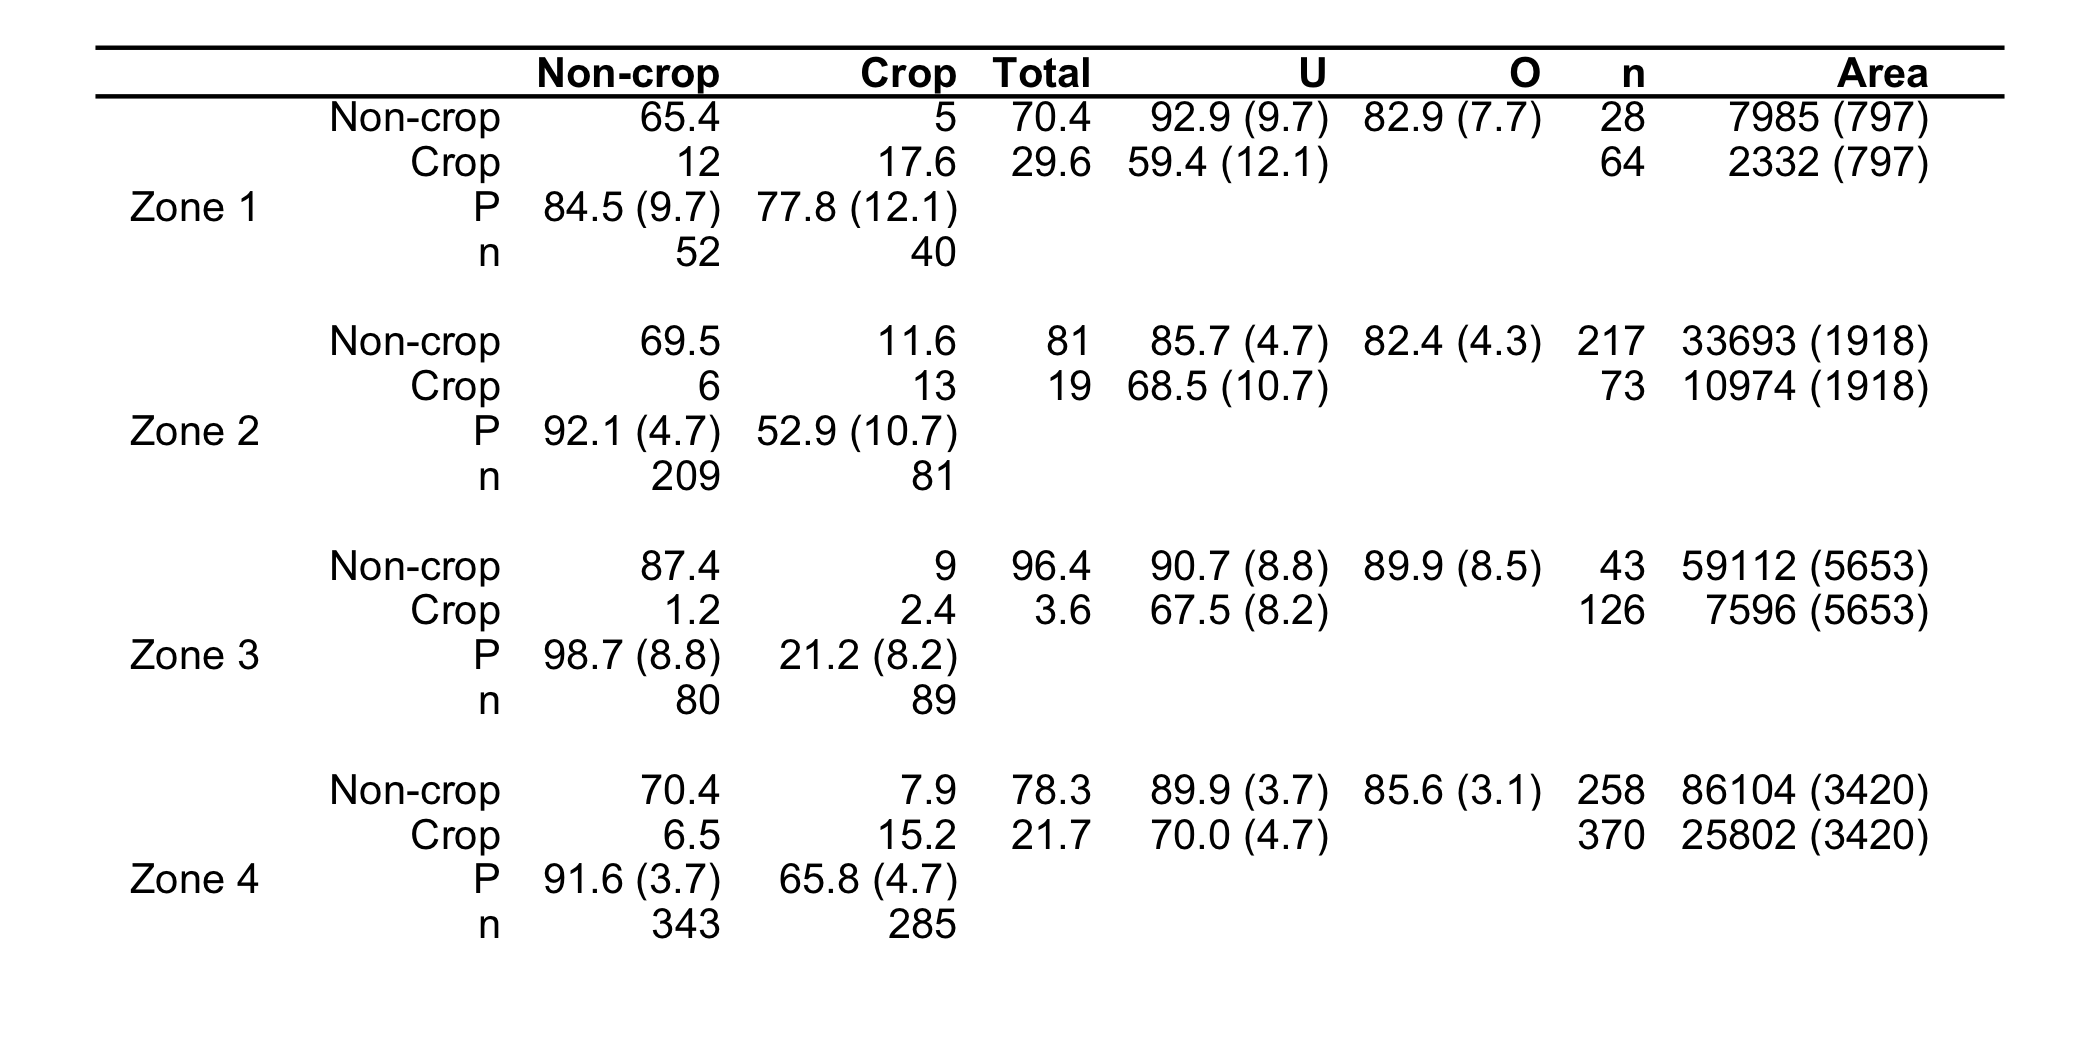
\includegraphics[width = 16cm]{figures/si_aez_accuracies.png}
\end{center}
\label{tab:aezaccuracy}
\end{table}

\hypertarget{field-area-and-number}{%
\subsubsection{Field area and number}\label{field-area-and-number}}

To mean, median, and distributions of the average area of segmented
field boundaries over the 100 validation sites in each AOI are compared
to the areas of the polygons digitized by the most accurate labeller
over the same sites in Figure \ref{fig:areavalidation}. The same
statistics for average number of segments versus average number of
labelled polygons across validation sites in each AOI are shown in
Figure \ref{fig:numbervalidation}.\\

\begin{figure}[!ht]

{\centering 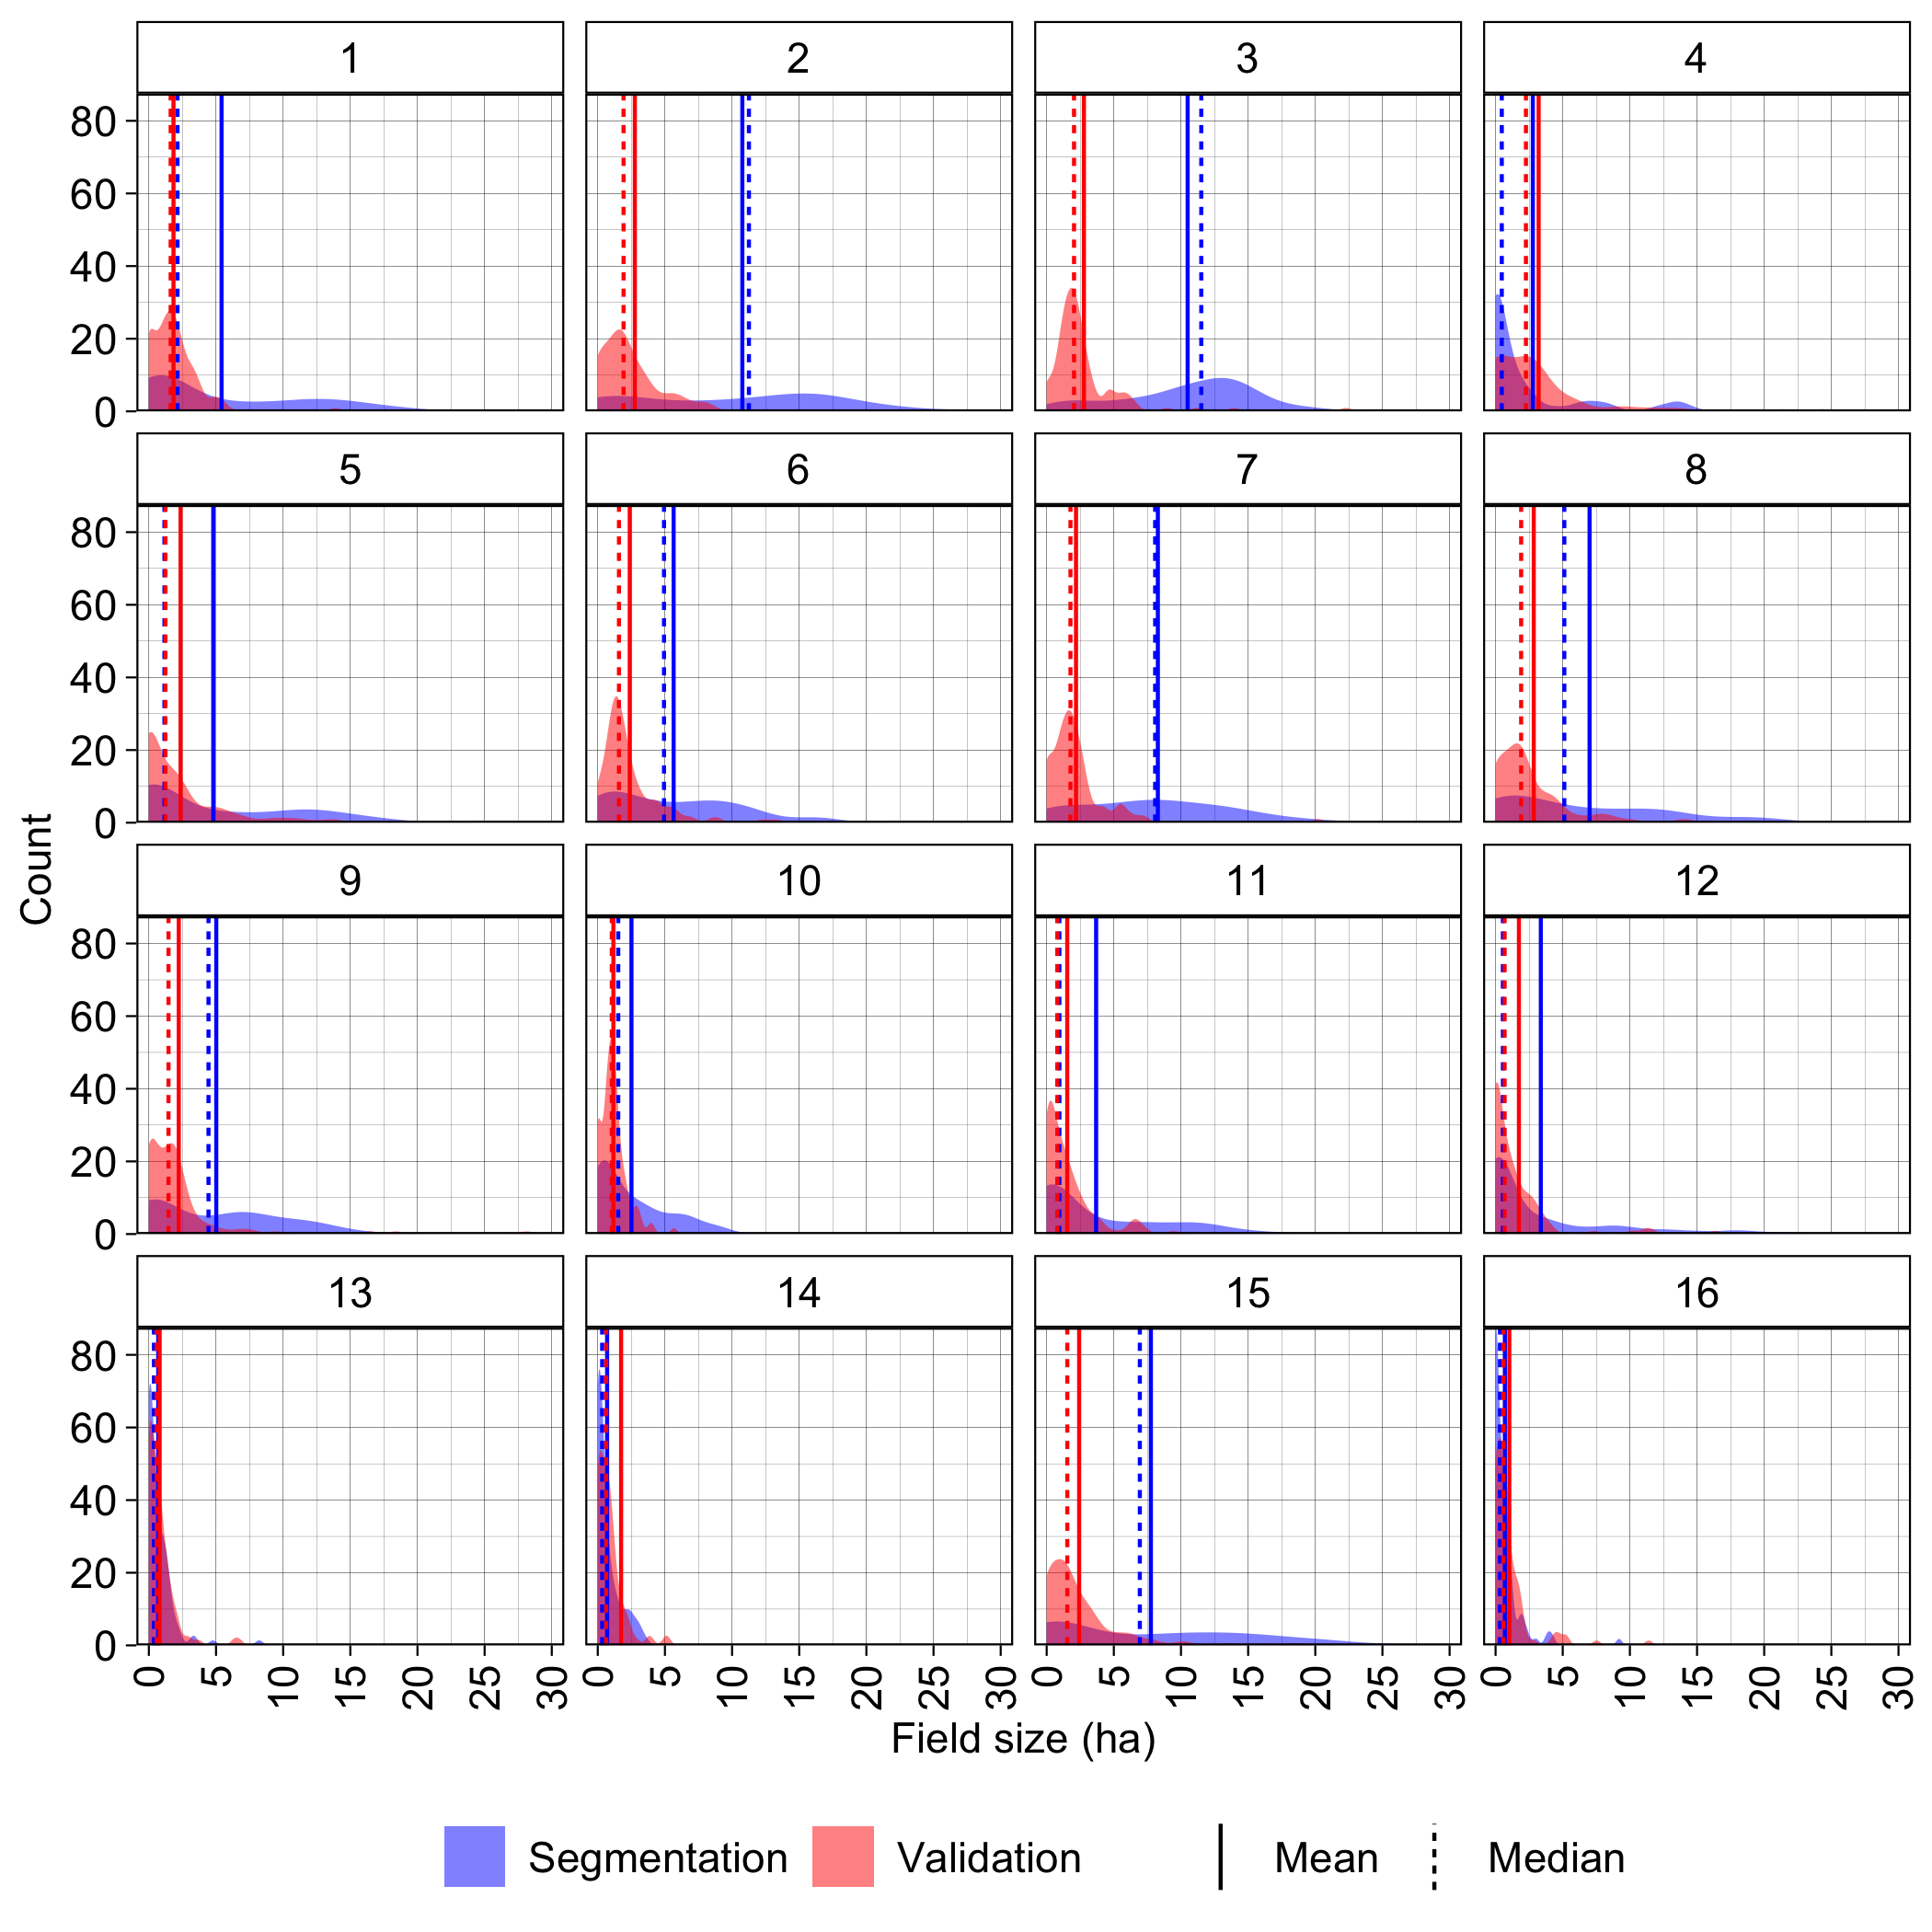
\includegraphics[width=0.9\linewidth,]{figures/si_validation_stats_fha2} 

}

\caption{The distributions of the average areas (in hectares) of segmented field boundaries (shown in blue) at the 100 validation sites per AOI, compared with the average areas of field boundaries digitized (shown in red) by the most accurate worker to label each site. Vertical lines indicate the mean and median of each distribution.}\label{fig:areavalidation}
\end{figure}

\begin{figure}[!ht]

{\centering 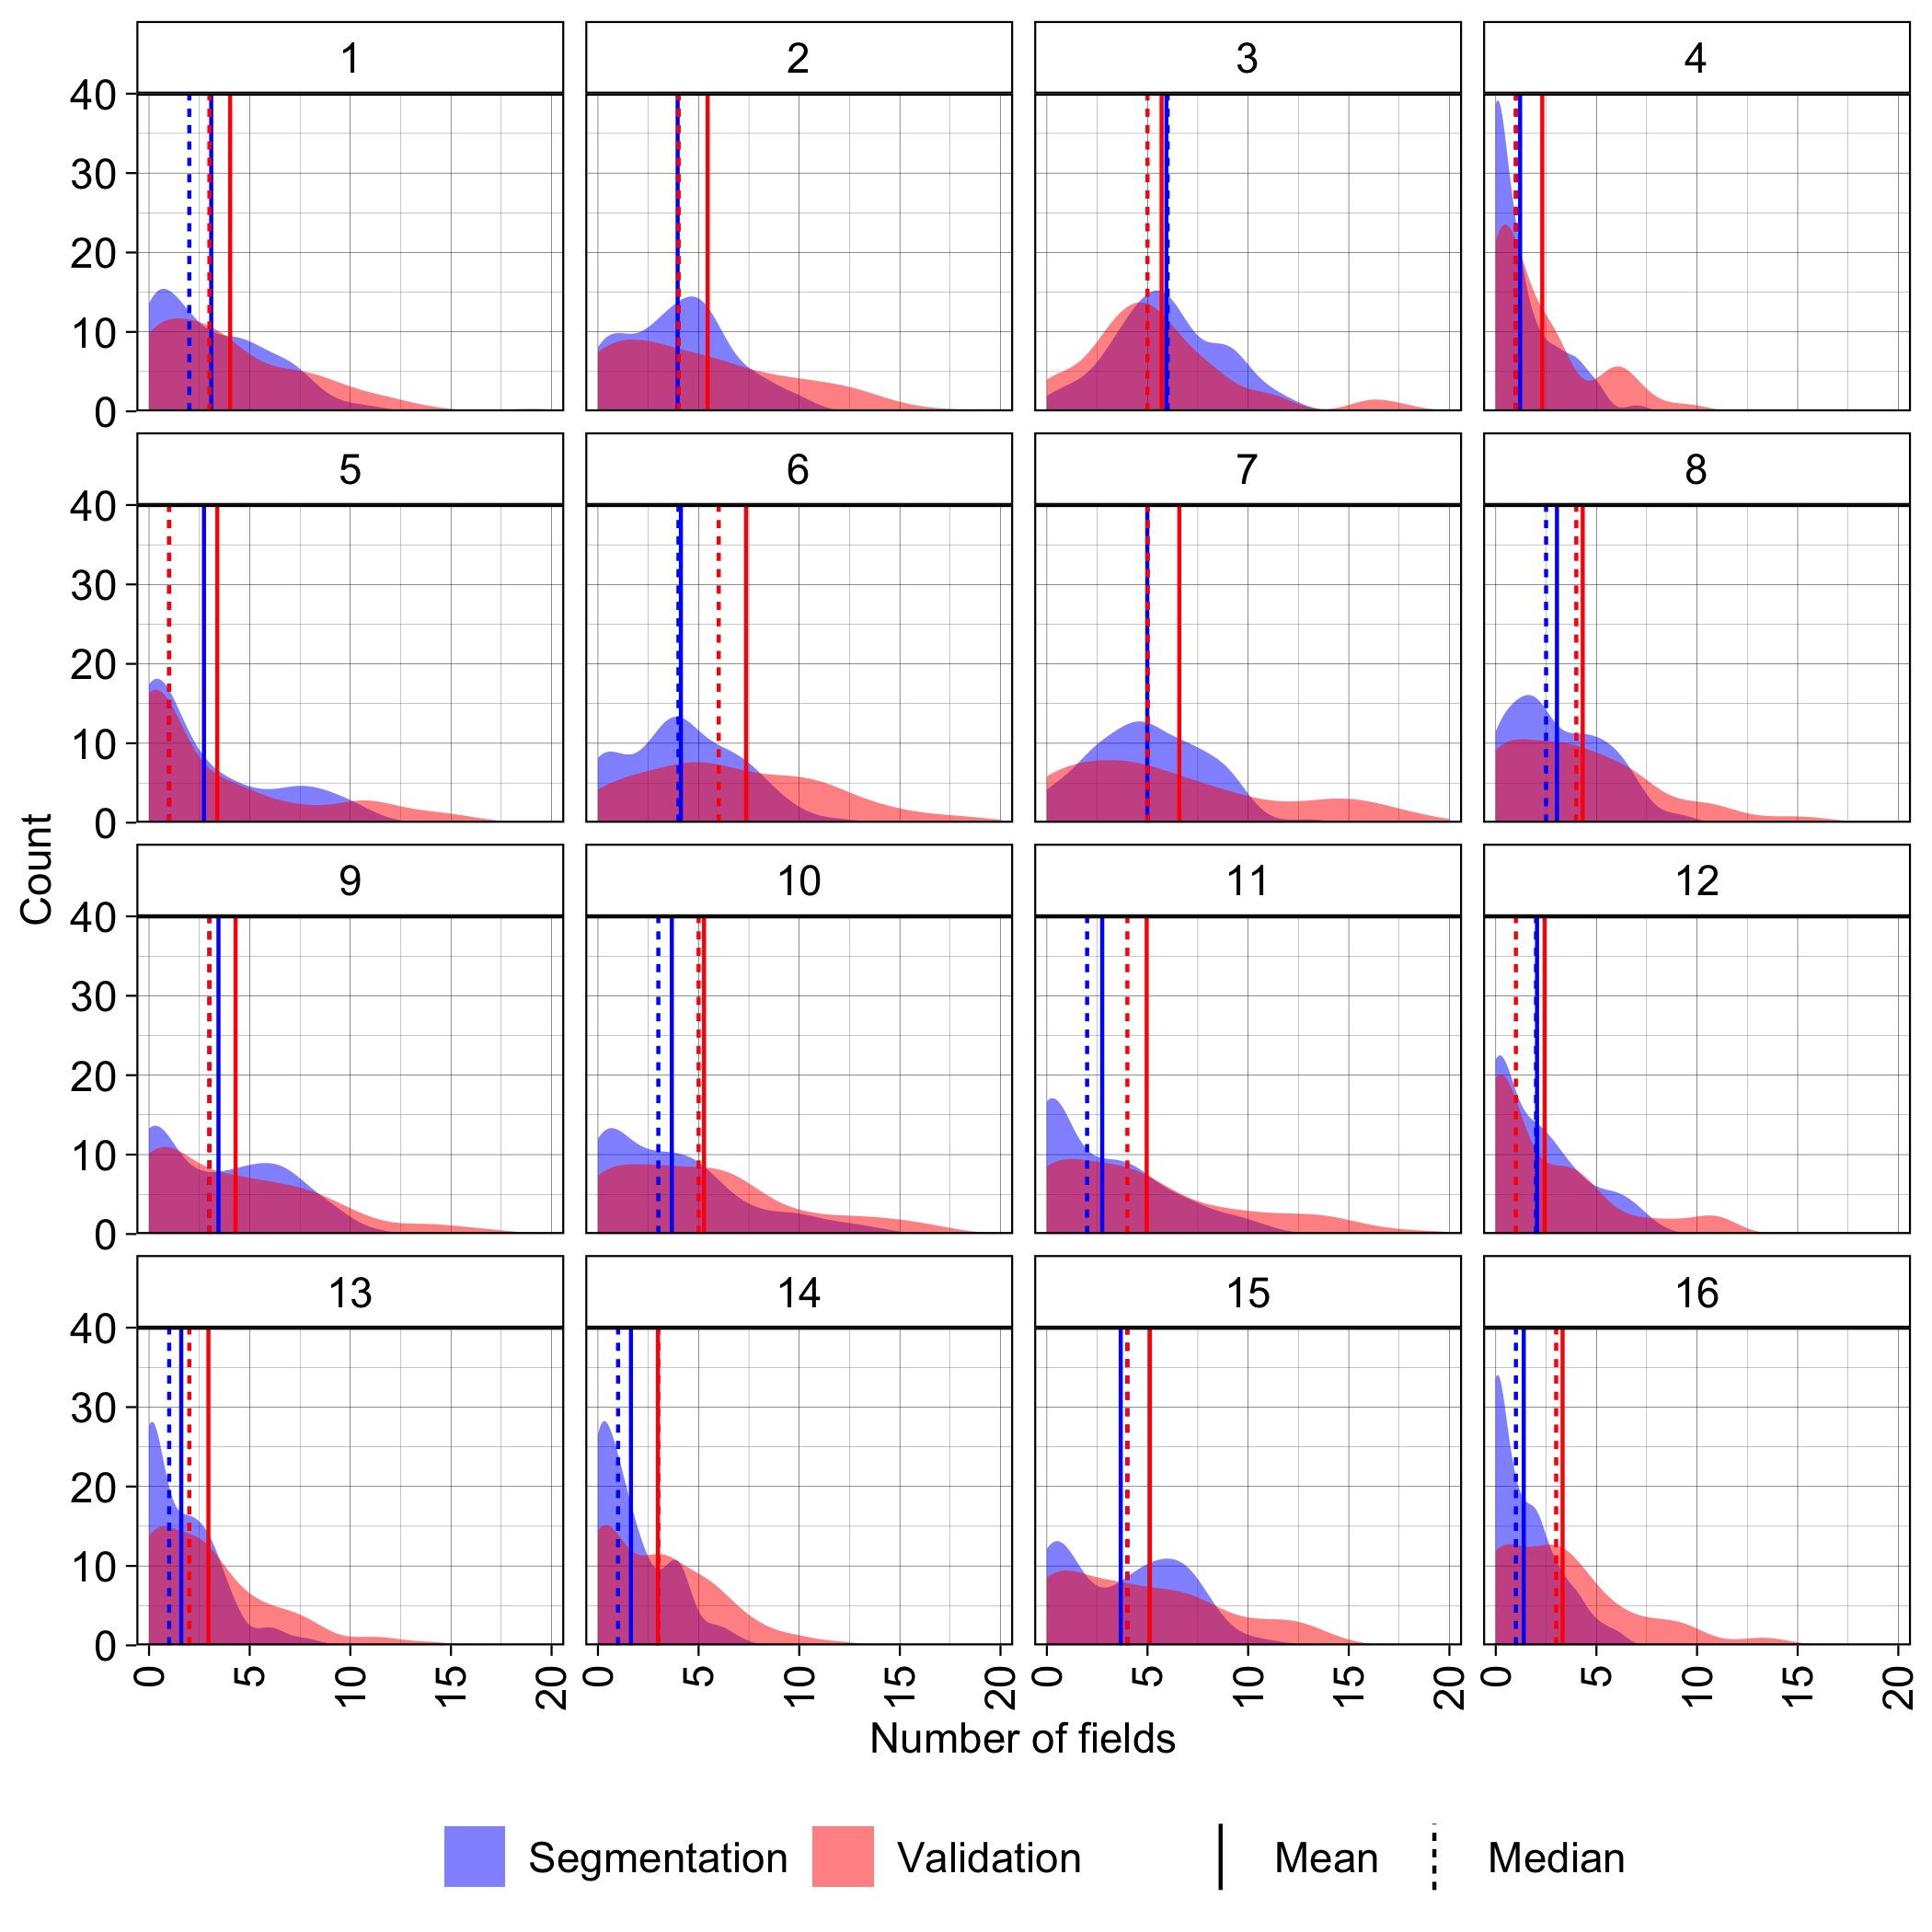
\includegraphics[width=0.9\linewidth,]{figures/si_validation_stats_fn2} 

}

\caption{The distributions of the average number of segmented field boundaries (shown in blue) at the 100 validation sites per AOI, compared with the average number of digitized polygons (shown in red) by the most accurate worker to label each site. The mean and median of each distribution is shown. Vertical lines indicate the mean and median of each distribution.}\label{fig:numbervalidation}
\end{figure}

\hypertarget{cropland-characteristics}{%
\subsection{Cropland characteristics}\label{cropland-characteristics}}

\hypertarget{field-area-and-number-1}{%
\subsubsection{Field area and number}\label{field-area-and-number-1}}

To examine average field sizes, and the total number, the mean segment
size per 0.05 degree tiles was calculated and mapped, as well as the
total number of fields per tile (Figure \ref{fig:fieldsizes}).

\begin{figure}[!ht]

{\centering 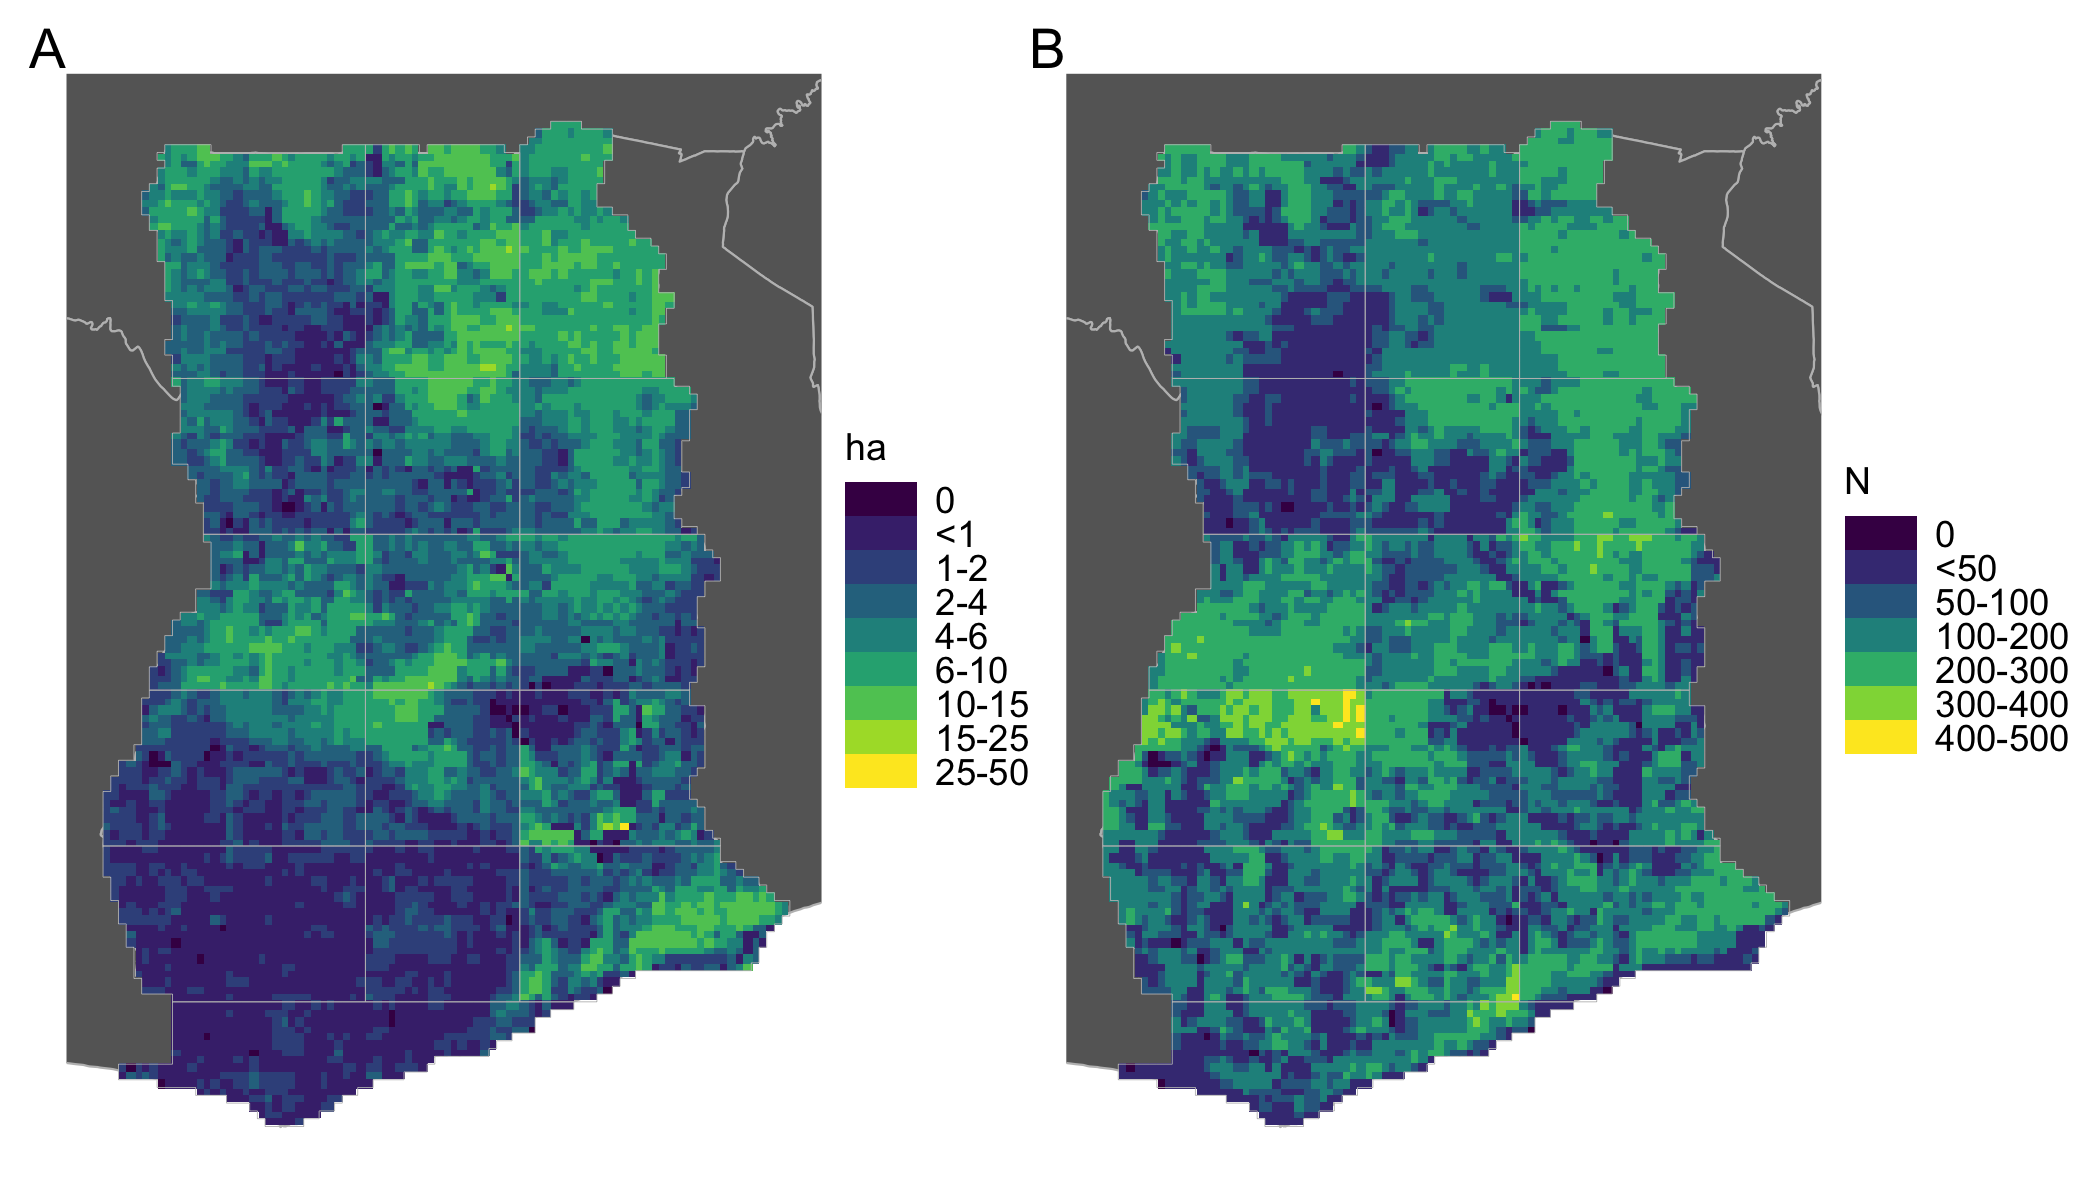
\includegraphics[width=0.9\linewidth,]{figures/si_fsize_n_05} 

}

\caption{The A) average sizes of fields and B) total number of fields in each 0.05 degree tile, as calculated from the vectorized field boundaries.}\label{fig:fieldsizes}
\end{figure}

\clearpage

\hypertarget{references}{%
\section{References}\label{references}}

\singlespace

\hypertarget{refs}{}
\begin{CSLReferences}{1}{0}
\leavevmode\hypertarget{ref-azaveaRasterFoundry2020}{}%
Azavea. 2020. Raster {Foundry}.
https://github.com/raster-foundry/raster-foundry.

\leavevmode\hypertarget{ref-hijmansRasterGeographicData2020}{}%
Hijmans, R. J. 2020. Raster: Geographic data analysis and modeling.
Manual.

\leavevmode\hypertarget{ref-pebesmaSimpleFeaturesStandardized2018}{}%
Pebesma, E. 2018. Simple features for r: Standardized support for
spatial vector data. The R Journal 10:439--446.

\leavevmode\hypertarget{ref-planetteamPlanetApplicationProgram2018}{}%
PlanetTeam. 2018. Planet application program interface: In space for
life on {Earth}. {https://api.planet.com}, {San Francisco, CA}.

\leavevmode\hypertarget{ref-StehmanKeyissuesrigorous2019}{}%
Stehman, S. V., and G. M. Foody. 2019. Key issues in rigorous accuracy
assessment of land cover products. Remote Sensing of Environment
231:111199.

\end{CSLReferences}

\eleft

\clearpage

\end{document}
